% !TeX spellcheck = en_US
\documentclass[RAIstudentthesis%      style
              ,optCharter%            font
              ,optBlackHeadings%      black sections to reduce number of colored pages
              ,optBlackRefs%          black references to reduce number of colored pages
              %,optCMYK%              color model
              ,optBiber% 	          bibliography tool
              ,optBibstyleAlphabetic% bibliography style
              ,optCenterEquations%    alignment of equations
              ,optEnglish% 		      language
              %,optTikzExternalize%   compiles faster for large tikz images
              %,optExzellenz%
              ]{RAIlatex}
%
% Load other LaTeX packages
\usepackage{booktabs}
\usepackage{graphicx}
\usepackage{textcomp}%
%
% Set paths
\graphicspath{{figures/}}%
\addbibresource{chapters/literature.bib}%
%
% Define additional commands
\newcommand{\code}[1]{\texttt{#1}}%
\newcommand{\degree}[0]{^\circ}%
%
\begin{document}%
% Titlepage
% ---------
\frontmatter%
% Info: separate multiple supervisors by \newline
%\RAIstudentthesisTitlePageCustomDiplomarbeit{German Title}{English Title}{\RAIlangFieldOfStudyRoboticsCognitionIntelligence}{Martin Mustermann}{}{\RAInamesProfKnoll}{Musterbetreuer, M.Sc.}{\RAIutilsDate{1}{1}{2020}}%
%\RAIstudentthesisTitlePageCustomBachelorsThesis{German Title}{English Title}{\RAIlangFieldOfStudyRoboticsCognitionIntelligence}{Martin Mustermann}{}{\RAInamesProfKnoll}{Musterbetreuer, M.Sc.}{\RAIutilsDate{1}{1}{2020}}%
%\RAIstudentthesisTitlePageCustomSemesterThesis{German Title}{English Title}{\RAIlangFieldOfStudyRoboticsCognitionIntelligence}{Martin Mustermann}{}{\RAInamesProfKnoll}{Musterbetreuer, M.Sc.}{\RAIutilsDate{1}{1}{2020}}%
%\RAIstudentthesisTitlePageCustomIDP{German Title}{English Title}{\RAIlangFieldOfStudyRoboticsCognitionIntelligence}{Martin Mustermann}{}{\RAInamesProfKnoll}{Musterbetreuer, M.Sc.}{\RAIutilsDate{1}{1}{2020}}%
\RAIstudentthesisTitlePageCustomMastersThesis{Monokulare 3D Objekterkennung mit HD-Karten}{Monocular 3D Object Detection Using HD Maps}{\RAIlangFieldOfStudyInformatics}{Joseph Birkner}{}{\RAInamesProfKnoll}{Walter Zimmer, M.Sc.}{\RAIutilsDate{31}{3}{2023}}%
%
% Abstract
% --------
% In total max. 1 Page!
\RAIstudentthesisAbstract{%
%
% Abstract English:
Due to their low cost and high output information density, monocular RGB cameras are a popular sensor choice for many perception tasks, including 3D object detection. The low cost of the sensor is especially important for the large-scale deployment of road-side infrastructure, as envisioned by the Providentia project. Prior work within the project determined, that a two-stage detection approach using the bottom contour of $2D$ instance masks is viable in a highway setting. However, the applicability of the $2D \rightarrow 3D$ lifting approach via the mask in urban settings has been unclear. In this work, we propose an augmented L-Shape fitting algorithm which solves the monocular 3D object detection task for urban settings. The algorithm is augmented using HD maps to inform likely heading values, and tracking, to further improve the heading value selection. We evaluate our algorithm on the Providentia A9R1 urban scenario dataset. The augmented algorithm improves over basic L-Shape fitting by $22\%$ in \textit{mAP}, $8.36\%$ in \textit{IoU}, and reaches $5.37\degree$ of orientation error and $0.9m$ in translation error. We conclude, that the approach is useful for real-time application in road-side infrastructure sensing tasks.
}{%
%
% Zusammenfassung Deutsch:
Aufgrund ihrer geringen Kosten und hohen Informationsdichte sind monokulare RGB-Kameras eine beliebte Sensorwahl für viele Wahrnehmungsaufgaben, einschließlich der 3D-Objekterkennung. Die niedrigen Kosten des Sensors sind besonders wichtig für den großflächigen Ausbau von straßenseitiger Infrastruktur, wie er im Rahmen des Providentia-Projektes vorgesehen ist. Frühere Arbeiten im Rahmen des Projekts ergaben, dass ein zweistufiger Erkennungsansatz, der die untere Kontur von $2D$-Objektinstanzmasken verwendet, für den Einsatz an Autobahnen geeignet ist. Unklar blieb jedoch die Anwendbarkeit dieses $2D \rightarrow 3D$ Lifting-Ansatzes in städtischen Szenarien. In dieser Arbeit schlagen wir einen erweiterten L-Shape-Fitting Algorithmus vor, der die Aufgabe der monokularen 3D-Objekterkennung auch in diesen Szenarien löst. Der Algorithmus wird durch HD-Karten erweitert, um wahrscheinliche Ausrichtungswinkel zu ermitteln, und durch Tracking, um die Selektion der Ausrichtungswinkel weiter zu verbessern. Wir evaluieren unseren Algorithmus anhand des Providentia A9R1-Datensatzes für urbane Szenarien. Der erweiterte Algorithmus verbessert das grundlegende L-Shape-Fitting um $22\%$ in \textit{mAP}, $8.36\%$ in \textit{IoU}, und erreicht sowohl $5.37\degree$ Rotationsfehler als auch $0.9m$ Positionsfehler. Wir kommen zu dem Schluss, dass der Ansatz für die Echtzeitanwendung für 3D-Sensoren an der straßenseitigen Infrastruktur geeignet ist.
}
%
%
% Content
% -------
\RAIstudentthesisPrintTableOfContents%
\mainmatter%
% !TeX spellcheck = en_US

\chapter{Acknowledgements}
\label{ch:ack}

I would like to thank my thesis advisor Walter Zimmer for his relentless pursuit of perfection for our monocular perception algorithms, as well as Suren Sritharan, wo completed some essential groundwork towards adopting SORT and L-Shape-Fitting into our codebase.

% !TeX spellcheck = en_US

\chapter{Introduction}
\label{ch:intro}

\section{The Providentia++ Project}
\label{sec:providentia}

The Providentia Project~\cite{krammer2022providentia} aims to create a large-scale Intelligent Infrastructure System (IIS) that can provide autonomous vehicles and traditional vehicles with complementary information about each road user and the overall traffic situation.
By observing and detecting all road users from multiple perspectives, an IIS can greatly extend a vehicle's perception range, enabling it to plan its maneuvers more safely and proactively.
The primary goal of Providentia is to improve the safety and comfort of autonomous vehicles by reducing their reliance on on-board sensors and providing them with a better and spatially extended understanding of their surrounding scene.

There are several related projects in the field of IIS, including the Test Area Autonomous Driving Baden-Württemberg, the MEC-View project, and the local highway operator in Austria's road operator system~\cite{DBLP:journals/corr/abs-2112-05615}.
While these projects have similar goals, they are smaller in scale than Providentia and use different sensor types.
Additionally, many research contributions propose methods of making algorithmic use of the information provided by an IIS, or optimizing their function.

Providentia uses a combination of multimodal sensors, including radars, LIDARs, and cameras.
The radars and LIDARs provide distance measurements and can detect objects that are out of the camera's field of view.
The cameras capture a more distant environment than the LIDARs, but objects that are too far away appear small on the image and cannot be reliably detected.
The combination of these sensors provides redundant road coverage with overlapping field of views, accurate calibration, and robust detection and data fusion algorithms.

The RGB camera sensor captures visual information about the environment, which is used to generate the digital twin.
It can capture a more distant environment than the LIDARs but is prone to severe occlusions due to its low perspective.
The RGB camera sensor is essential for fusing multiple sensor perspectives and updating the digital twin, which includes information such as position, velocity, vehicle type, and a unique identifier for every observed vehicle.
By providing this digital twin to an autonomous driving research vehicle, Providentia demonstrates that it can be used to extend the limits of the vehicle’s perception far beyond its on-board sensors.
The update rate for the digital twin depends on the fusion-setup and the type of the used object detection network, and it can vary between 13.1Hz to 24.6Hz depending on the sensor setup.

% ----------------------------------------------------

\section{The A9 Testfield}
\label{sec:a9testfield}

\begin{figure}[htb]
    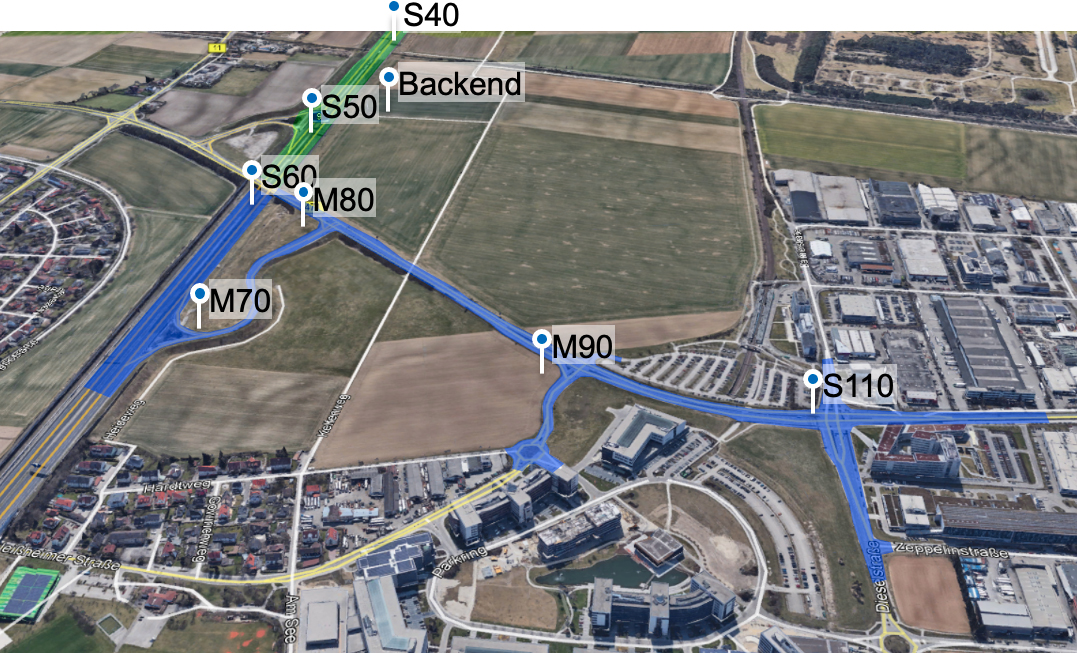
\includegraphics[width=\linewidth]{figures/teststrecke-gesamt}
    \caption{Overview of the Providentia A9 Test Stretch (Graphic produced using Google Maps).}
    \label{fig:providentia-test-area}
\end{figure}

At the heart of the Providentia Project is an expansive test area with multiple sensor stations.
The sensor stations are each equipped with RGB Camera, LIDAR and RADAR sensors.
These are used to test the sensor calibration-, road user detection-, sensor-fusion-, tracking-, and communication-solutions that are developed as part of the project.
An overview of the test area along the A9 highway near Garching Hochbrück, Germany is provided in Figure~\ref{fig:providentia-test-area}.

This work focuses on the RGB Camera sensors, which are installed at the designated stations.
The goal of this work is to develop a perception algorithm which can calculate a three-dimensional digital twin of any visible road user from the two-dimensional RGB camera input frames.
Previous work on the Monocular 3D Object Detection (\textit{Mono3D}) task in the scope of Providentia focused on solving this task for the sensor stations along the A9 highway~\cite{leonthesis}: \texttt{S40}, \texttt{S50} and \texttt{S60}.
In this work, we aim to generalize the Mono3D solution to cover the more urban sensor stations, in particular the cameras which are installed at the \texttt{S110} intersection.
This urban intersection setting is more challenging, because it does not allow for a fixed orientation of road users to be assumed by the monocular detector.
Instead, the detector must induce a contextual bias for each road user to determine their orientation angle.

Crucially, a high-definition (HD) map of the test area was also developed as part of the Providentia project using the OpenDRIVE format~\cite{dupuis2010opendrive}.
An overview of the map with a more detailed view of the S110 intersection is provided in Figure~\ref{fig:providentia-opendrive-map}.
Within this project, we aim to explore how the HD map of the test area can serve as  auxiliary sensory input to monocular detector.
We hypothesize, that the highly detailed map might provide the monocular detector with information about viable road user orientations.

For the demonstration purpose of this work, we focus our efforts on two cameras which are installed at the S110 sensor station: \texttt{S110-S1} and \texttt{S110-S2}.
Both cameras have a native resolution of 1920x1200 pixels, run at 60 Hz, and have a 90 degree field of view.  % TODO: Determine Correct FOV!

\begin{figure}[htb]
    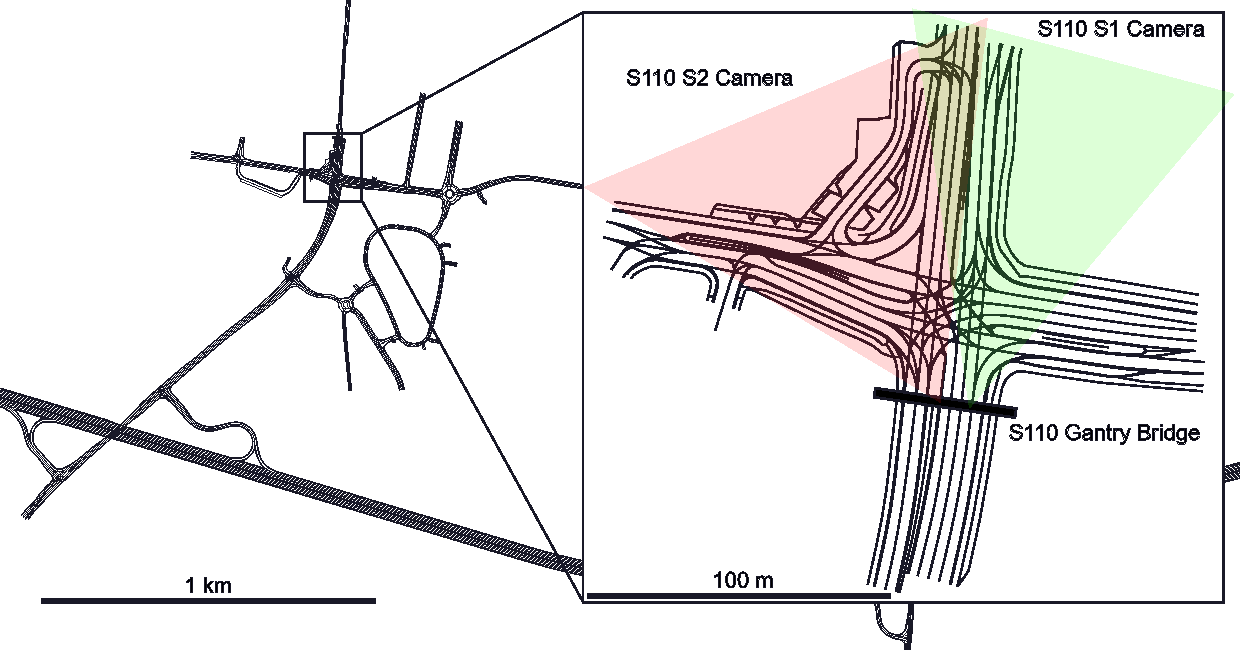
\includegraphics[width=\linewidth]{figures/map}
    \caption{Overview of the OpenDRIVE map of the Providentia test area, with zoomed in cut-out of the S110 intersection with its S1 and S2 cameras.}
    \label{fig:providentia-opendrive-map}
\end{figure}

% ----------------------------------------------------

\section{The A9R1 Dataset}
\label{sec:a9dataset}

In order to evaluate any object detection method, labeled data are required.
For this purpose, the \textit{A9R1} dataset was developed under the umbrella of Providentia.
The dataset annotates both LIDAR point-clouds with categorized 3D object bounding boxes, and RGB Camera frames with 2D cuboid labels.
Specifically, four scenes in the dataset provide the crucial combination of 3D LIDAR bounding box labels for 2D camera frames.
This labeling pair allows us to evaluate our monocular 3D object detector.
The four scenes in the dataset which do provide this required annotation mode are listed in table~\ref{tab:a9r1}.

\begin{table}[h]
    \centering
    \caption{A9R1 dataset scenes which provide camera frames annotated with 3D detection bounding boxes from LIDAR labels.}
    \label{tab:a9r1}
    \begin{tabular}{llllll}
        \toprule
        Scene & Perspective & \#Frames & \#Detections & Weather & Time of Day \\
        \midrule
        Scene 4 & S110 Camera S1 & 300 & XXXXX & Sunny & Daytime \\
        Scene 4 & S110 Camera S2 & 300 & XXXXX & Sunny & Daytime \\
        \midrule
        Scene 5 & S110 Camera S1 & 300 & XXXXX & Sunny & Daytime \\
        Scene 5 & S110 Camera S2 & 300 & XXXXX & Sunny & Daytime \\
        \midrule
        Scene 8 & S110 Camera S1 & 1200 & XXXXX & Sunny & Daytime \\
        Scene 8 & S110 Camera S2 & 1200 & XXXXX & Sunny & Daytime \\
        \midrule
        Scene 9 & S110 Camera S1 & 619 & XXXXX & Rain & Night \\
        Scene 9 & S110 Camera S2 & 619 & XXXXX & Rain & Night \\
        \bottomrule
    \end{tabular}
\end{table}

The dataset frame-rate is 10 Hz. The combination of 3D LIDAR Labels and RGB camera frames introduces an additional challenge in the form of synchronization delay \textemdash there may be up to 200 ms of difference between the 2D RGB frame and the 3D LIDAR annotation timestamps.
We will discuss this problem in more detail in Chapter~\ref{ch:evaluation}.
Each road user is also annotated with a category; one of \texttt{CAR}, \texttt{BUS}, \texttt{TRUCK}, \texttt{VAN}, \texttt{MOTORCYCLE}, \texttt{BICYCLE}, \texttt{PEDESTRIAN}, \texttt{EMERGENCY\_VEHICLE}, or \texttt{OTHER}.

% ----------------------------------------------------

\begin{figure}[htb]
    \includegraphics[width=\linewidth]{figures/mono3d}
    \caption{\textbf{On the left:} General dataflow in the Monocular 3D Object Detection task. For each instance of a recognized object in the RGB input frame, the detector must estimate a 3D pose parameter-set. The more variables the detector must estimate, the harder the task becomes. For example, elevation (i.e. the position z component) may be omitted. \textbf{On the right:} Figure 4.4 from~\cite{leonthesis}. Frame of a highway scene. In such a scenario, the detector may also omit the calculation of the heading (yaw) orientation angle and assume a fixed value.}
    \label{fig:mono3d-task-overview}
\end{figure}

\section{Monocular 3D Object Detection}
\label{sec:monodet}

\subsection{Estimands}
\label{subsec:estimands}

Monocular 3D Object Detection (\textit{Mono3D}) is the process of detecting three-dimensional objects from a single two-dimensional RGB camera output frame.
However, the term \textit{3D Object Detection} might be misleading in the context of this work.
In reality, the number of variables which a \enquote{3D} object detector may derive for an object far surpasses three, as can be seen in the following table~\ref{tab:mono3d-variables}.

\begin{table}[h]
    \centering
    \caption{Parameterization options for the output of a Monocular 3D Object Detector per object.}
    \label{tab:mono3d-variables}
    \begin{tabular}{lll}
        \toprule
        Variable & Description & Optional \\
        \midrule
        $X$/$Y$ & Position along the longitudinal/lateral axes.\ & \textbf{No} \\
        \midrule
        $L$/$W$ & Extent (length/width) along the longitudinal/lateral axes.\ & \textbf{No} \\
        \midrule
        $\delta X$/$\delta Y$/$\delta Z$ & Speed.\ Derivatives of the position/elevation variables.\ & \textbf{Yes} \\
        \midrule
        $Z$ & The elevation of the object over the road surface.\ & \textbf{Yes} \\
        \midrule
        $H$ & The height of the object.\ & \textbf{Yes} \\
        \midrule
        $\theta$ & Yaw (heading) angle, determines travel direction.\ & \textbf{No} \\
        \midrule
        $\phi/\gamma$ & Tilt/Roll angles, e.g.\ terrain slope or crash scenarios.\ & \textbf{Yes} \\
        \midrule
        $I$ & Identifier for the object across multiple frames.\ & \textbf{Yes} \\
        \midrule
        $C$ & Category of the object, e.g. \texttt{CAR} or \texttt{PEDESTRIAN}.\ & \textbf{No} \\
        \bottomrule
    \end{tabular}
\end{table}

We observe, that a minimal 3D Object Detector should actually estimate six dimensions per object: Birds-eye-view (BEV) positions $X$/$Y$, BEV size $L$/$W$, heading angle $\theta$ and category $C$.
Earlier work on the \textit{Mono3D} task for the Providentia project~\cite{leonthesis} focused on solving this task for the highway scenario.
On top of the minimum six variables, this early detector also calculated the object height.
However, as the early detector focused on the highway scenario, it was able to assume a fixed value for the $\theta$ variable.
This is illustrated on the right side of Figure~\ref{fig:mono3d-task-overview}.
As this work strives to generalize the \textit{Mono3D} solution beyond the highway, it must treat the $\theta$ value as non-fixed.
Interestingly, we facilitate this task by also estimating the identity $I$ variable, which then also allows us to estimate the planar speed $\delta X$/$\delta Y$ variables.
So we will end up with a 10-D detector in this work.

\subsection{Two-Stage Detection}
\label{subsec:twostage}

While many approaches are viable, the earlier Providentia \textit{Mono3D} detector by~\cite{leonthesis} used a so-called two-stage detection model.
As this work builds on top of~\cite{leonthesis}, we use the same approach.
Generally, the two-stage detector splits the detection task into two separate steps: a $2D$ instance segmentation step, and a $3D$ lifting step.
There are again many implementation options for these individual steps.
The steps are illustrated in Figure~\ref{fig:mono3d-two-stage}

\begin{figure}[htb]
    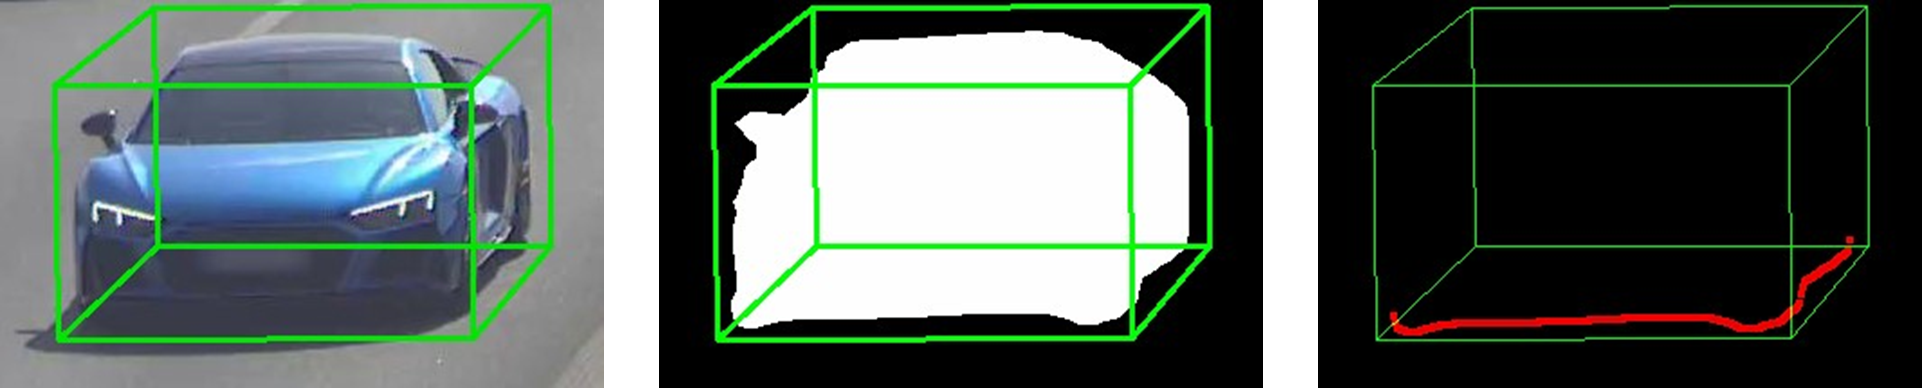
\includegraphics[width=\linewidth]{figures/two-stage-detection}
    \caption{Two-stage detection from camera image (left) via instance segmentation (middle) and $2D \rightarrow 3D$ lifting via the instance mask bottom contour (right). Graphic from~\cite{leonthesis}.}
    \label{fig:mono3d-two-stage}
\end{figure}

Within the taxonomy provided by \cite{survey2022}, these are also called \textit{Result-based Lifting Methods}. The primary advantage of this idea is that the 3D detector can benefit from highly polished, interchangeable, off-the-shelf instance segmentation models.
For example, the~\cite{leonthesis} detector exchanged \textit{Mask-RCNN}~\cite{he2017mask} in favor of \textit{Yolact-Edge}~\cite{liu2021yolactedge} in the first stage for performance reasons.
In this work we switch again, from \textit{Yolact-Edge} to \textit{YOLOv7}~\cite{wang2022yolov7} to improve the detection quality.
Another benefit is that stage two, the $2D \rightarrow 3D$ lifting stage, can be independently optimized, as the problem shifts from identifying the image areas occupied by relevant objects to estimating the three-dimensional properties of these objects.
The method proposed by~\cite{leonthesis} of lifting the $2D$ mask into $3D$ space via a $3D$ projection of the instance mask's bottom contour is applied and refined in this work.

The biggest hurdle towards a correct $3D$ vehicle pose estimation in an urban setting was identified by~\cite{leonthesis} as the $\theta$ (heading/orientation) value calculation.
The process by which an orientation angle can be estimated from the bottom contour is called \textit{L-Shape-Fitting}~\cite{zhang2017efficient}.
The vehicle bottom contour, which we want to use as an input to this calculation, can be quite noisy for many reasons, such as visual obstructions, upstream instance mask detection errors, or cropping at the image border (just to name a few).
Hence, an additional contextual bias is required for each object to correctly estimate its orientation angle.

\subsection{Use of Neural Networks}
\label{subsec:neural}

A Neural Network would most likely be a great choice for an algorithm to estimate not just the vehicle orientation $\theta$, but to perform the whole $2D \rightarrow 3D$ lifting stage.
For example, \textit{UrbanNet}~\cite{carrillo2021urbannet} implemented this approach with a Neural Network trained on synthetic data.
For this work, we are staying with a \enquote{rule-based}, non-neural approach for three reasons:

\begin{enumerate}
    \item Research continuity: The bottom-contour-based two-stage approach proposed by~\cite{leonthesis} is undoubtedly viable, there is no obvious reason to change the research direction.
    \item Explainability, Extendability, Maintainability: The \enquote{rule-based} approach allows for diagnosing and fixing particular failure modes.
    This is much harder with a neural network.
    \item Performance: A neural network estimator would most certainly require GPU resources to perform adequately in a real-time setting as required by the Providentia IIS. On the other hand, the non-neural approach can function purely on the CPU, leaving the sparse GPU resources to other tasks.
\end{enumerate}

For these reasons, this work explores exclusively non-neural \enquote{Software 1.0} \footnote{\hyperlink{https://karpathy.medium.com/software-2-0-a64152b37c35}{https://karpathy.medium.com/software-2-0-a64152b37c35}} solutions for the $2D \rightarrow 3D$ lifting stage.

\section{Relevance of HD Maps}
\label{sec:hdmap}

High-definition (HD) maps model the road network down to the detail of individual driving lane geometries.
In this work, we hypothesize that the HD-map can serve as a useful additional sensor to the \textit{Mono3D} detector.
In particular, we explore whether the HD map can serve as a viable source of vehicle orientation (heading) values.
In the first step, we developed a method to derive the likely heading value at a particular position on the road surface from the geometry of the enclosing lane boundaries.
This method is described with more detail in Chapter~\ref{sec:hdmapgrids}.
By converting the calculated $\overrightarrow{xyz}$ heading vectors at each position to $\text{RGB}$ colors, we are able to proof the general idea.
This is visualized in Figure~\ref{fig:headings-color-coded}.

\begin{figure}[htb]
    %\begin{tabular}{lll}
    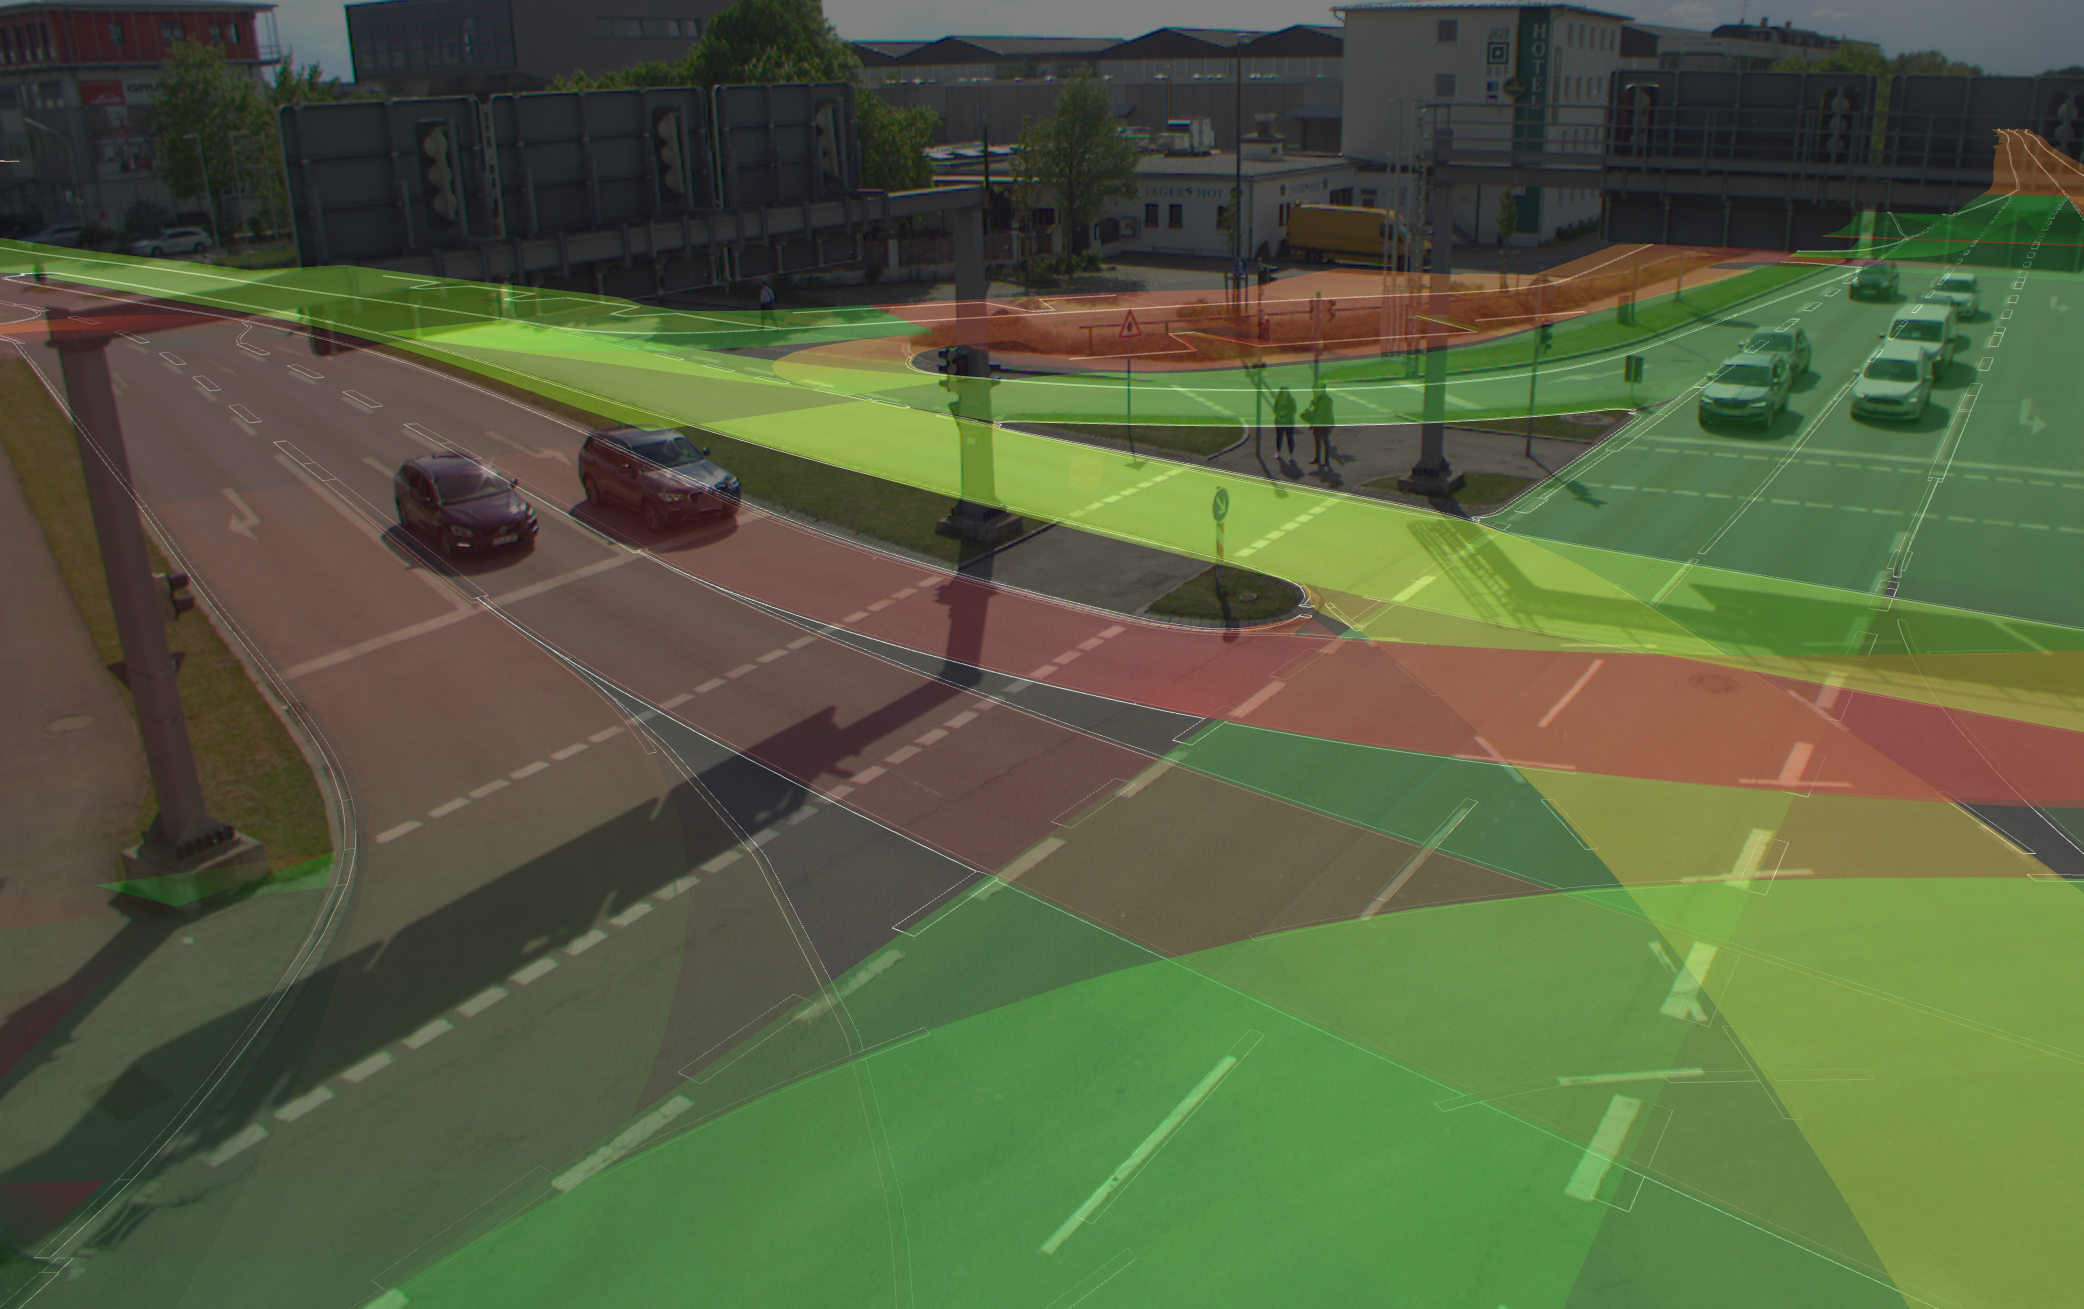
\includegraphics[width=0.4\linewidth]{figures/headings-colored-s2} % &
    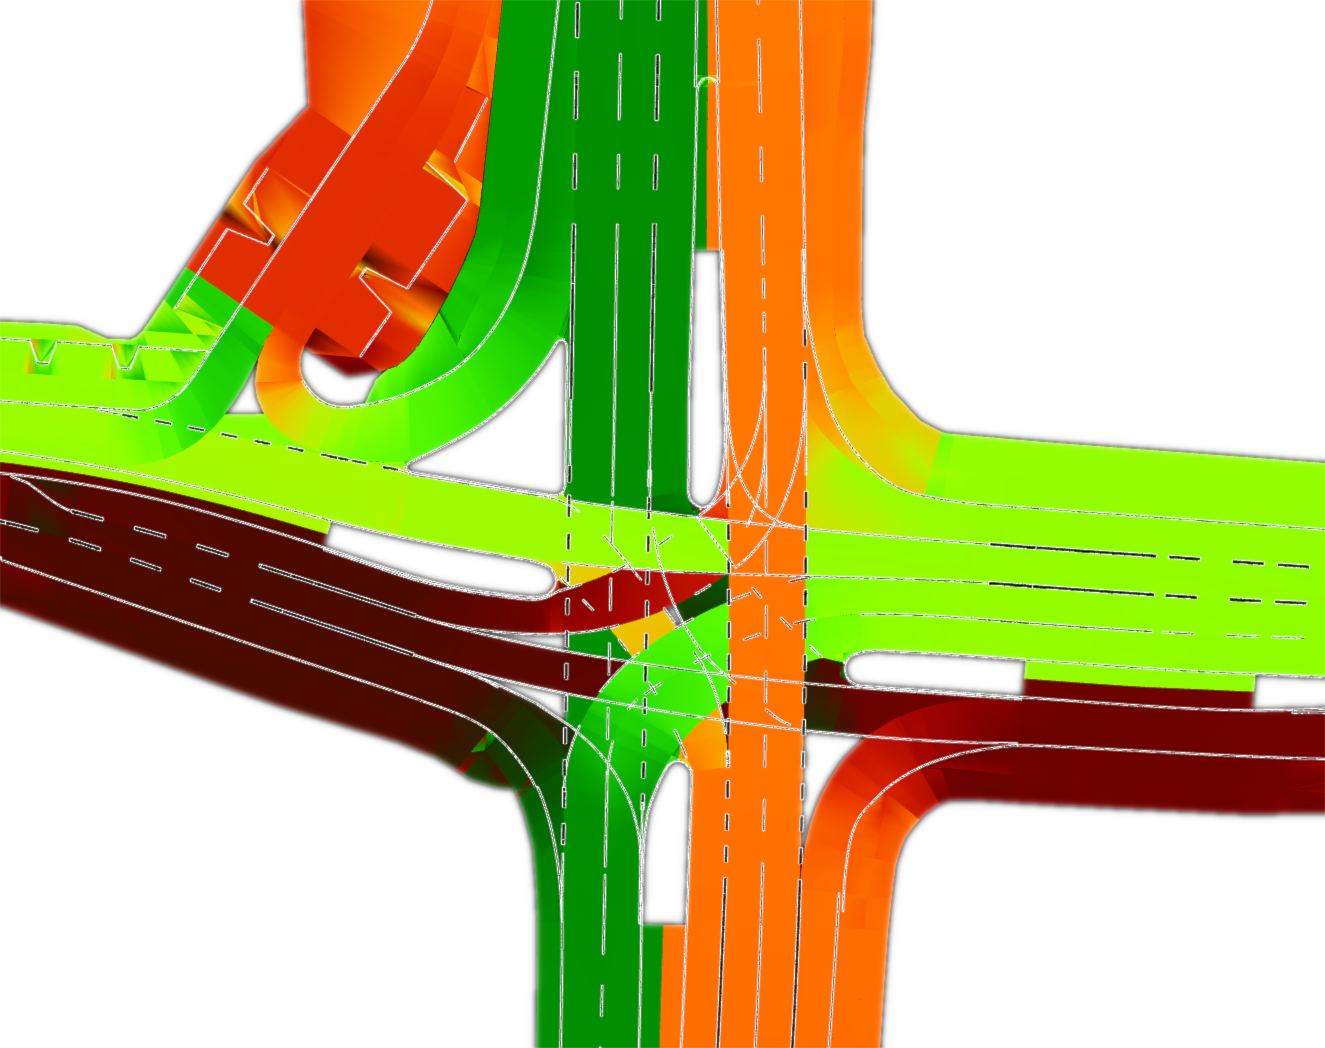
\includegraphics[width=0.29\linewidth]{figures/hdmap-heading-s110}
    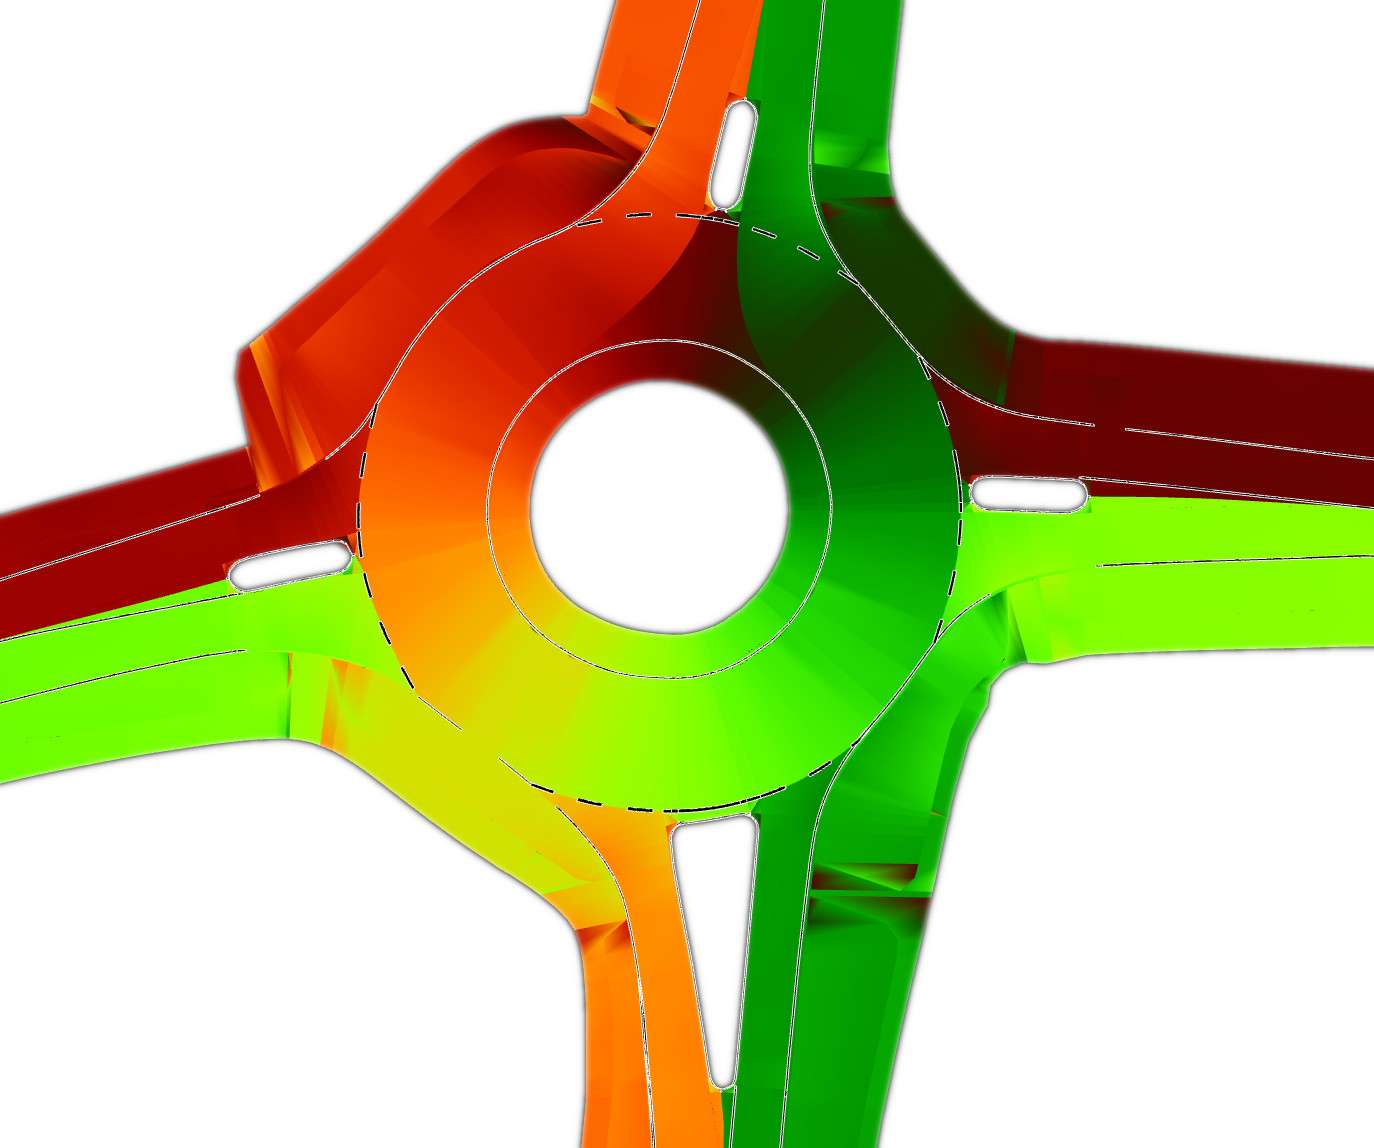
\includegraphics[width=0.29\linewidth]{figures/hdmap-heading-roundabout} % &
    %\end{tabular}
    \caption{Visualisation of heading vectors as RGB values, smoothly interpolated from the lane boundary geometry. \textbf{Left:} Colored heading overlays for the S110-S2 camera perspective. In the bottom-right corner, there are four overlapping lanes. \textbf{Middle:} RGB heading visualization for the whole S110 intersection. \textbf{Right:} RGB heading visualization for a roundabout.}
    \label{fig:headings-color-coded}
\end{figure}

From this proof-of-concept visualization of the heading vectors, it becomes apparent that the map-derived headings may serve well as an additional per-pixel feature for the \textit{Mono3D} detector.
But it also becomes apparent, that there may always be many possible overlapping heading options provided by the HD map, as there may always be many overlapping lanes \textemdash especially in the context of urban intersection scenarios.
The left-most image of Figure~\ref{fig:headings-color-coded} illustrates this problem quite well.
Here we see color-coded headings overlaid on top of a frame from the \texttt{S110-S2} camera.
Towards the bottom-right corner of the image, there are locations with up to four overlapping lanes, which provide four distinct heading options!
Therefore, an additional information source is needed to resolve ambiguities among multiple heading options.

% ----------------------------------------------------

\section{Tracking Enters the Picture}
\label{sec:tracking}

\subsection{Screen-Space Tracking}
\label{subsec:sstracking}

In face of the aforementioned uncertainties when deciding between ambiguous heading options, it might be useful to consider previously known spatial orientations of a vehicle.
Consider a scene such as the one shown in Figure~\ref{fig:tracking}.

\begin{figure}[htb]
    \centering
    \includegraphics[width=0.7\linewidth]{figures/tracking}
    \caption{Visualisation of a \textit{Mono3D} detection scenario where tracking resolves a heading ambiguity.}
    \label{fig:tracking}
\end{figure}

In this scene, the \textit{Mono3D} detector $C$ observes the instance mask of vehicle $M$.
Through the screen-space bounding box of $M$, the detector is able to associate this instance mask with detections from previous frames \textemdash $P_0$ and $P_1$.
The mask $M$ also allows for the calculation of the 3D position $P_2$.
The detector then performs a lookup for $\theta$ (heading) options at location $P_2$, and obtains two possible headings: $\theta_1$ and $\theta_2$.
As the detector must now pick one of these heading options, it may use the given knowledge of previous historical positions ($P_0$ and $P_1$) for $M$ to bias towards $\theta_1$ as the more likely orientation.
This is, because the detector assumes that vehicles move in a continuous direction more often than not, and erratic turns are less likely than forward motion.

To express this intuition formally, given a detection $M$ at time $t$ which is associated with a set of historical positions $P=\{p_{t},\mathellipsis,p_{t-T}\}$, we wish to pick $\theta(M)$ such that \[\sum_{\delta=1}^{\delta=T} |\theta(M) - \text{atan2}(p_t - p_{t-\delta})|\] is minimal.
In this work, the storage and retrieval of historical positions for the screen-space bounding box of a detection is accomplished using the \textit{SORT}~\cite{bewley2016simple} object tracking algorithm.

\subsection{Birds-Eye-View Tracking}
\label{subsec:bevtracking}

We use screen-space tracking to aid in the ranking of heading options.
However, the same tracking algorithm can also be used at a later stage for a different pupose:
In Birds-Eye-View \textit{(BEV)} tracking, objects are tracked in $3D$ space on the $X$/$Y$ axes rather than in camera image space.
This is where the \textit{Kalman-Filters}~\cite{welch1995kalman} which are at the heart of the \textit{SORT}~tracking algorithm really develop their potential as denoisers of physical measurements.
Fully implemented, they could denoise every variable of a tracked detection.
However, in this work, we will only use them to stabilize position and speed estimates.

\section{Inherent Functional Limitations}
\label{sec:limits}

As the origins, goals and methods of this work are now introduced, we can already identify functional limitations which are going to be inherent to our approach.
These limitations must be tackled by future work (see Chapter~\ref{ch:future}).

\begin{enumerate}
    \item \textbf{Bad detection quality for road users with highly cropped or obstructed instance masks}: Both the bottom-contour based L-Shape-Fitting algorithm, and the estimation of the vehicle position from the instance mask require an unobstructed full view of the road user to function optimally.\ Any obstruction of the view will degrade the estimation quality.\ Such an obstruction may be a stationary object in front of the road user, another road user, a weather condition like snow/rain/fog, or simply the field-of-view \textit{(FOV)} limit of the sensor.
    \item \textbf{Bad detection quality for road users in legal or physical peril:} Our \textit{Mono3D} detection approach assumes that road users do not fly, do not lie on their side, do not move sideways, and are always aligned with a legal traffic flow direction as parsed from the HD-map.\ Therefore, the 3D pose estimation for any road user which violates one of these assumptions will be as bad as the the day this road user is probably experiencing.
\end{enumerate}

\section{Research Objective}
\label{sec:objective}

In summary, the research objective for this work is to address the truthfulness of the following hypothesis: \textit{A two-stage \textit{Mono3D} detector with an instance-mask bottom-contour based estimator in the second stage can only function well within an urban intersection setting, if and only if the estimator is assisted by additional information from an HD map}.

\section{Contributions}
\label{sec:contributions}

This work presents the following research contributions:

\begin{enumerate}
    \item An Augmented L-Shape-Fitting Algorithm which supports tracking and HD-Map confidence inputs.
    \item A lookup strategy for vehicle bottom contours within the HD Map to derive Yaw Options with associated confidence values.
    \item An HD-Map Rasterization Algorithm to support fast bulk lookup of heading options for a vehicle bottom contour.
    \item A formula to derive the plausibility of a yaw hypothesis for a detected vehicle from a series of historical positions for the same vehicle.
    \item An algorithm to calculate the physical position and height of a vehicle, given its instance mask height and physical width/length.
    \item An algorithm to calculate 3D bounding boxes for Vulnerable Road Users (Pedestrians and Bicycles) from their Instance Mask Bottom Contour.
\end{enumerate}

% !TeX spellcheck = en_US

\chapter{Related Work}
\label{ch:related}

\section{Earlier Work Within the Providentia Project}
\label{sec:related-leon}

This work is deeply rooted in the earlier groundwork which was laid out for the \textit{Mono3D} task in highway scenarios~\cite{leonthesis} in the scope of the Providentia project.
Our earlier work took inspiration from the \textit{Cooperative Vehicle Infrastructure System}~\cite{guo2021detection} in the design and implementation of the two-stage detector based on the bottom contour of the vehicle instance mask, but also differs in key aspects.
The detection flow of our early \textit{Mono3D} highway detector is illustrated in Figure~\ref{fig:related-leon}.

\begin{figure}[htb]
    \centering
    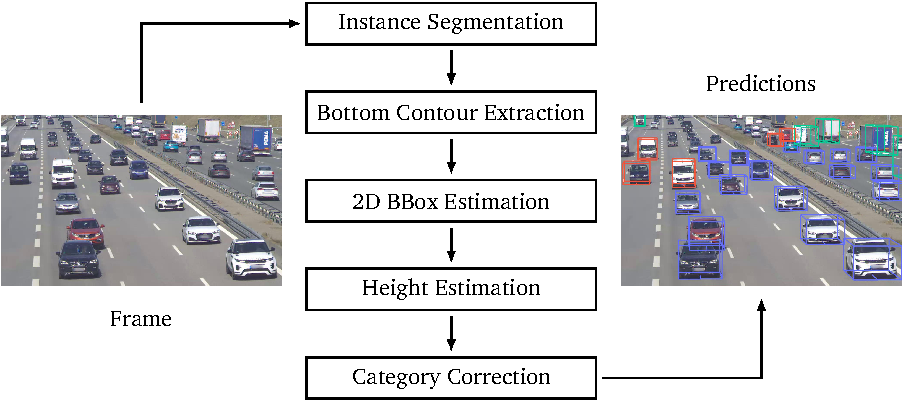
\includegraphics[width=0.9\linewidth]{figures/thesis_leon_fig_4_1}
    \caption{Figure 4.1 from~\cite{leonthesis}, illustrating the stages of the monocular 3D detection process for highway scenes.}
    \label{fig:related-leon}
\end{figure}

Note, that while this work adopts the first two elements of the detection flow \textemdash \textit{Instance Segmentation} and \textit{Bottom Contour Extraction} \textemdash we have completely reengineered all subsequent processes.
This earlier detector works well on highways because it assumes a fixed orientation for all vehicles.
This also allows for a very straight-forward linear equation to solve for vehicle heights given their distance from the camera, as well as their instance mask heights.
In this work, the vehicle orientation is dynamically derived from the HD map and the vehicle's positional history.
The height estimation algorithm is revised accordingly.

\section{Detection of Vehicles in Cooperative Vehicle Infrastructure Systems}
\label{sec:related-coopvis}

The earlier Providentia highway detector was inspired by the \textit{Cooperative Vehicle Infrastructure System (CVIS)}~\cite{guo2021detection}, which also uses a two-stage detector with a $2D \rightarrow 3D$ lifting stage based on the vehicle bottom contour.
Their approach is illustrated in Figure~\ref{fig:related-cvis}.

\begin{figure}[htb]
    \centering
    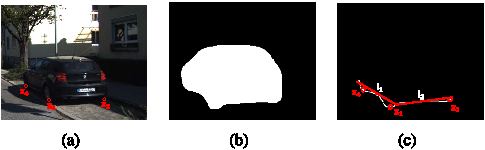
\includegraphics[width=1.0\linewidth]{figures/cvis_figure}
    %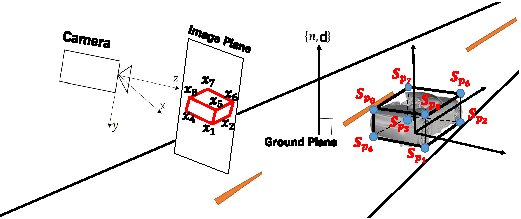
\includegraphics[width=0.39\linewidth]{figures/cvis_figure_2}
    \caption{Figure 1 from~\cite{guo2021detection}, illustrating their approach to keypoint estimation based on two lines which are regressed to the vehicle bottom contour: \textit{(a)} RGB image; \textit{(b)} vehicle segmentation mask; \textit{(c)} the contour point of the bottom edge of the vehicle and the contact points between vehicle and ground are represented by white dots and red circles.}
    \label{fig:related-cvis}
\end{figure}

While their approach has provided the basis for our research on \textit{Mono3d} in the Providentia project, it exhibits some flaws which we are hoping to have overcome (to some extent) in this work:

\begin{enumerate}
    \item Previous frames are not considered when a vehicle pose is estimated, potentially leading to bad yaw angle choices in ambiguous situations.
    \item They do not mention the effects of shadows or noise due to obstructions or weather on their bottom contour line regression algorithm.\ The L-Shape-Fitting algorithm which is used in this work might be more robust in such situations, especially since we also apply \textit{DBSCAN}-based outlier filtering on the bottom contour.
    \item Their height estimation solution assumes that the closest vehicle top corner and bottom corner share the same distance from the camera, which leads to \textit{leaning} boxes in traffic monitoring situations where the camera is stationed highly above the vehicles.
    \item They do not consider non-vehicle \textit{Vulnerable Road Users (VRUs)} in their detector, such as bicyclists or pedestrians.\ This work is also detecting VRUs.
\end{enumerate}

Finally, no code was published alongside their approach.
This inherently necessitates research to reproduce their results.

\section{The L-Shape Fitting Method for Vehicle Pose Detection}
\label{sec:related-lshape-fitting}

Branching off \textit{CVIS}, this work (like~\cite{leonthesis}) makes use of \textit{L-Shape-Fitting (LSF)} to estimate vehicle size and orientation from the instance mask bottom contour.
This approach can also be interpreted as a \textit{pseudo-lidar}~\cite{survey2022} approach because the back-projection of the instance mask bottom contour yields a (very flat) point-cloud.
Underlining the \enquote{LiDAR-esque} origins of the LSF algorithm is the fact that it was introduced in the scope of an object detection method from LiDAR measurements, in the work \textit{The L-Shape Fitting Method for Vehicle Pose Detection from LiDAR}~\cite{zhang2017efficient}.
Their method is illustrated in Figure~\ref{fig:related-lsf}.

\begin{figure}[htb]
    \centering
    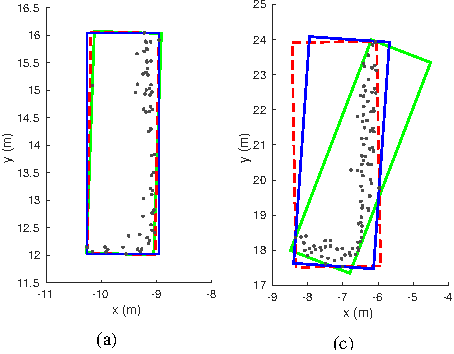
\includegraphics[width=0.49\linewidth]{figures/l_shape_fitting_fig_2_1-cropped}
    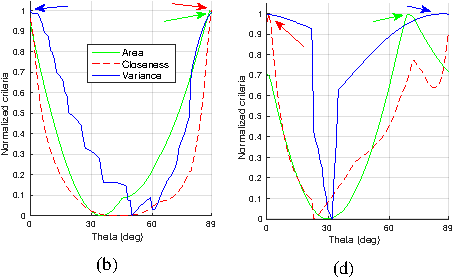
\includegraphics[width=0.49\linewidth]{figures/l_shape_fitting_fig_2_2-cropped}
    \caption{Figure 2 from~\cite{zhang2017efficient}. In (a) and (c), the grey dots represent the laser range scan points and the rectangles in green, red, and blue are the fitted rectangles by using criteria area minimization, closeness maximization, and variance minimization. The normalized scores for the three criteria over the searched directions are plotted in (b) and (d), respectively. In example (a), the fitting results from the three criteria are very similar, and the maxima of the three curves in (b) are very close (marked by arrows and achieved at 88◦, 89◦, and 0◦, respectively). In example (b), the fitting result from the area criteria is different from the other two, and its maximum in (d) is away from the other two (achieved at 69◦, 1◦, and 86◦, respectively).}
    \label{fig:related-lsf}
\end{figure}

By regressing a rectangular shape to the bottom contour, the LSF algorithm can estimate orientation, BEV position and BEV size simultaneously.
The regression is performed by maximizing one of three error criteria: \texttt{Area}, \texttt{Closeness} or \texttt{Variance}.
The algorithm and the criteria are explained in section~\ref{sec:lshapefitting}.
In this work, we further adapt and develop this approach to stabilize size and heading estimates in complex traffic observation scenarios using tracking and the HD map.

\section{TrafficNet}
\label{sec:related-trafficnet}

The \textit{TrafficNet} detector~\cite{rezaei2021traffic} is a very thorough two-stage monocular traffic monitoring solution, encompassing both vehicle and VRU detection, tracking, speed estimation, and even road geometry prediction from satellite images.
This is illustrated in Figure~\ref{fig:related-tranet}.

\begin{figure}[htb]
    \centering
    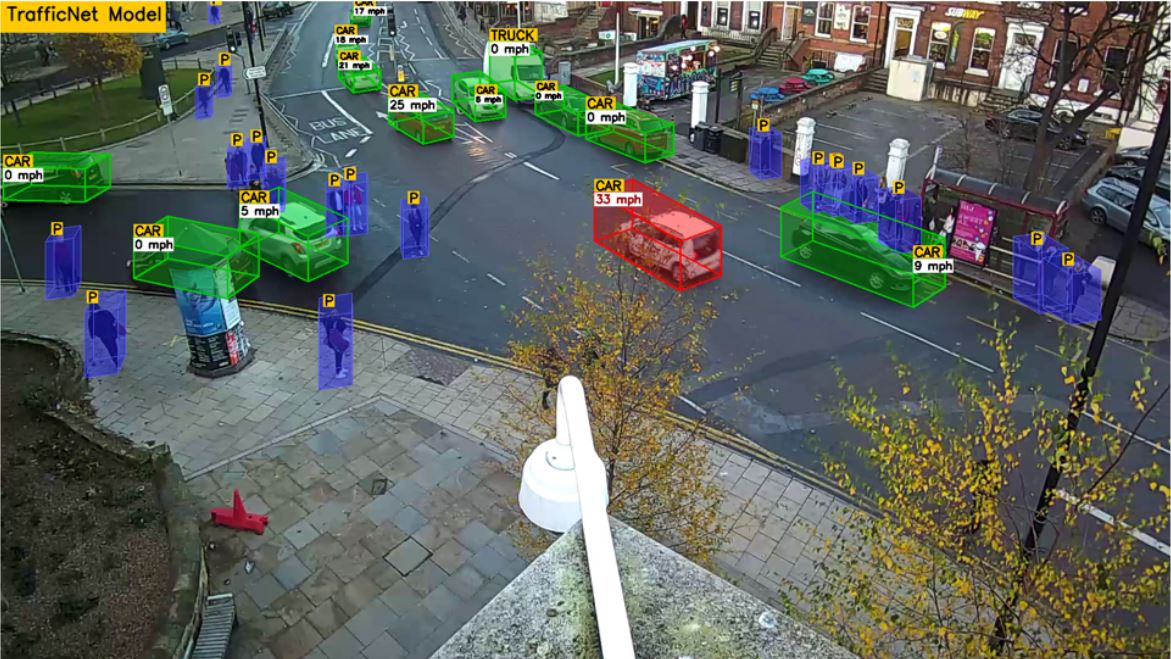
\includegraphics[width=0.63\linewidth]{figures/tranet}
    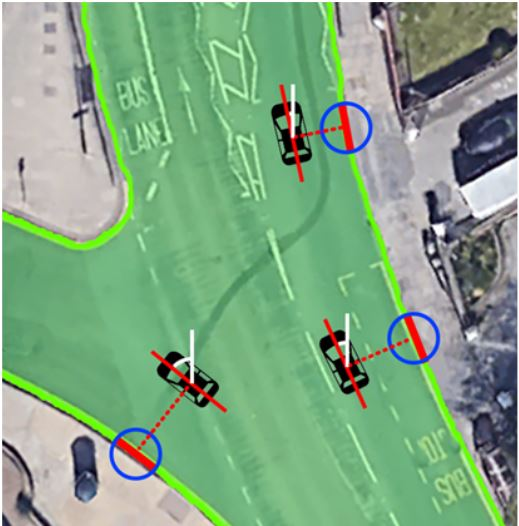
\includegraphics[width=0.35\linewidth]{figures/tranet-angle-estimation}
    %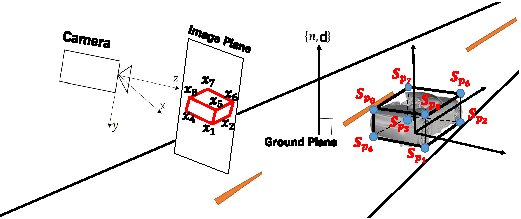
\includegraphics[width=0.39\linewidth]{figures/cvis_figure_2}
    \caption{Figures 12 and 13(c) from~\cite{rezaei2021traffic}, illustrating their approach to heading estimation based on the geometry of proximate road curbs which have been extracted from sattelite imagery. This is analogous to our use of the HD map in this work (to some extent).}
    \label{fig:related-tranet}
\end{figure}

As can be seen from the right side of Figure~\ref{fig:related-tranet}, they make use of road curb geometry which is extracted from a satellite image to make estimates of vehicle headings, substituting the role of the HD map in this work.
Note that heading estimation via the most proximate curb would not be applicable in this work, as curbs within a complex intersection with many overlapping lanes are not a good indicator of orientation.
However, their approach alleviates the need for rather hard-to-source high-definition maps, which is a point of weakness in this work.
Another strong point of \textit{TrafficNet} is their extensive use of Kalman Filters~\cite{welch1995kalman} to de-noise the vehicle poses and category estimations.
They also fine-tuned a custom instance mask segmentation model in the first detector stage based on YOLOv5~\cite{glenn_jocher_2020_4154370}.
This is done both to detect additional object categories, and to speed up inference by removing convolutions which are only needed to detect large objects.
One weak point of their work is the extensive use of \enquote{magic values} in the second detector stage: They make use of pre-defined sizes based on vehicle categories and calculate 3D object height based on a pre-calculated factor of \textit{$0.6$} from the instance mask height.
Also, unfortunately, no code is publicly available for \textit{TrafficNet}.

\section{UrbanNet: Urban Maps for Long Range 3D Object Detection}
\label{sec:related-urbnet}

Another case of a two-stage object detector which uses Urban maps to augment the performance of the $2D \rightarrow 3D$ lifting-stage is \textit{UrbanNet}~\cite{carrillo2021urbannet}.
This solution is unique, because it applies the HD map as an auxiliary feature to a small Feed-Forward Neural Network.
The architecture is illustrated in Figure~\ref{fig:related-urbnet}.

\begin{figure}[htb]
    \centering
    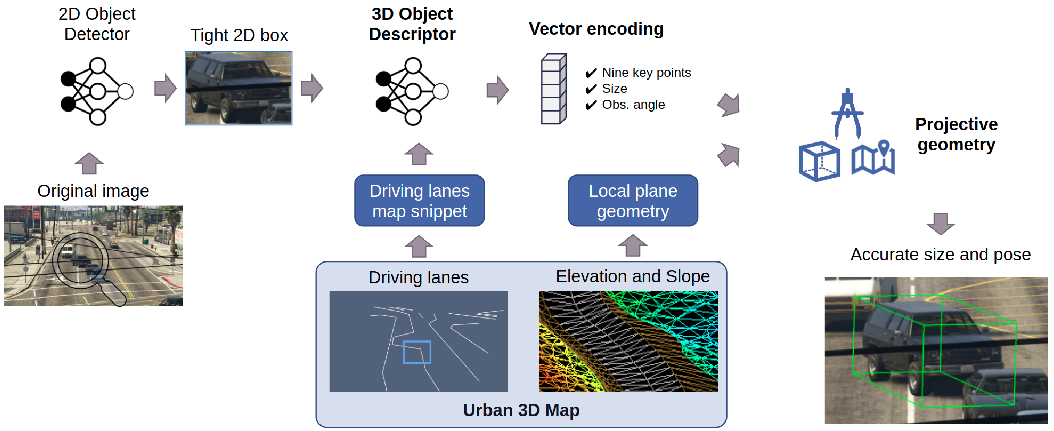
\includegraphics[width=1.0\linewidth]{figures/urbannet_architecture}
    \caption{Figure 2 from~\cite{carrillo2021urbannet}, describing how the Urban HD map assists the 3D object descriptor estimation model. Center-lines are \textit{painted} as a per-pixel feature into the 3D object descriptor network's single input image.}
    \label{fig:related-urbnet}
\end{figure}

This approach provides an interesting way to remediate some of the shortcomings of L-Shape-Fitting in the second detector stage.
The neural network can learn to recognize obstructed road user poses, or even highly uncommon poses, such as a car laying on its side in a crash scenario.
This is not possible with a bottom-contour based detector.
Furthermore, the runtime performance of this approach might be overall better than ours, as there is no requirement for the first detector stage to output and compute expensive per-instance image masks.
Notably, they also incorporate slope estimation into their prediction, which is especially useful for long-range vision in mountainous terrain.
The bottleneck in this case is the availability of training data, something which is solved in UrbanNet by training and testing exclusively on artificial computer-generated road scenes.

\section{Cooperative Roadside Vision Systems in Complex Scenarios}
\label{sec:related-crvis}

Finally, the \textit{Complex Scenario Cooperative Roadside Vision System}~\cite{masi2021augmented} is related as prior work due to its two-stage monocular 3D object detection architecture and usage of HD maps in all stages of the detection processes.

\begin{figure}[htb]
    \centering
    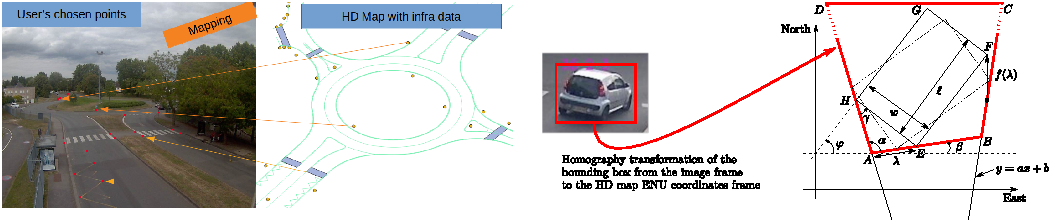
\includegraphics[width=1.0\linewidth]{figures/coop_roadside_vis_aug_perception_fig}
    \caption{Figures 2 and 3 from~\cite{masi2021augmented}, describing how the HD map is used for calibration (left) and how the vehicle size is calculated from its 2D bounding box (right).}
    \label{fig:related-crvis}
\end{figure}

Their system uses the HD map for calibration (as illustrated in Figure~\ref{fig:related-crvis}), heading calculation, and tracking.
On the other hand, their paper is not clear on when and how exactly they make use of the HD-map for heading estimation.
In some or most cases, they fall back to a projection of the 2D screen-space bounding box onto the 3D ground plane, from which a vehicle's BEV width/length and heading may be calculated.
They do not make any attempts at calculating vehicle heights or detecting VRUs.

\section{Survey Studies}
\label{sec:related-surveys}

In the conclusion of this related work study, several survey papers were consulted, some of which shall be highlighted here for reference.
First, the survey \textit{3D Object Detection from Images for Autonomous Driving}~\cite{survey2022} was a great resource to learn a taxonomy for the multitude of architectural approaches towards the \textit{Mono3d} task.
Furthermore, the survey on \textit{Object Detection in Traffic Videos} provides an in-depth overview of the spectrum of techniques which are used in 2D object detection neural networks, such as YOLO~\cite{wang2022yolov7}.
Research on \textit{Infrastructure-Based Object Detection and Tracking for Cooperative Driving Automation}~\cite{bai2022infrastructure} is very connected to this work, and the cited survey includes many of the previously mentioned related works.
Finally, the \textit{Review on Cooperative Perception and Control Supported Infrastructure-Vehicle Systems}~\cite{yu2022review} is the only survey which mentions HD maps as an auxiliary data source and shared spatial reference frame for cooperating autonomous vehicles.

% !TeX spellcheck = en_US

\chapter{Technical Foundations}
\label{ch:tech}

This chapter provides additional technical details for specific algorithms and techniques that are later referenced in our System Design (Chapter~\ref{ch:system}). Feel free to skip this chapter if you are roughly familiar with the following methods: $2D$ object instance segmentation, the \textit{OpenDRIVE} and \textit{Lanelet2} map data formats, the \textit{Robot Operating System (ROS)}, the \textit{DBSCAN} point clustering algorithm, the \textit{SORT} object tracking algorithm, the \textit{L-Shape-Fitting} algorithm (as previously mentioned in Section~\ref{sec:related-lshape-fitting}), and common object detection evaluation metrics, such as \textit{mAP} and \textit{IoU}.

\section{The YOLACT Instance Segmentation Model}
\label{sec:yolact}

\textit{YOLACT (You Only Look at Coefficients)}~\cite{bolya2019yolact} is a real-time instance segmentation method that focuses on processing static images.
It simplifies the instance segmentation problem by separating it into two parallel tasks, enabling faster processing while maintaining competitive accuracy.
The functionality of \textit{YOLACT} can be described in three main steps (as illustrated in Figure~\ref{fig:yolact}):

\begin{enumerate}
    \item \textbf{Generating Prototype Masks:} \textit{YOLACT} employs a fully convolutional network called \textit{ProtoNet} to generate a fixed set of K prototype masks, which are used as the base for constructing the final object instance masks.\ These prototype masks are shared across all object instances in the image.
    \item \textbf{Predicting Per-instance Mask Coefficients and Bounding Boxes:} In parallel to generating prototype masks, \textit{YOLACT} predicts per-instance mask coefficients and bounding boxes for potential objects using an anchor-based approach.\ Each anchor is associated with a mask coefficient vector, which has the same length as the number of prototype masks (K). Additionally, the model predicts the class probabilities and bounding box coordinates for each anchor.
    \item \textbf{Assembling Final Instance Masks:} To obtain the final instance masks, \textit{YOLACT} linearly combines the prototype masks using the predicted mask coefficients.\ The model selects the top scoring instances based on their class probabilities and applies a non-maximum suppression (NMS) algorithm to remove duplicate detections.\ The result is a set of instance masks, each associated with a specific object class and bounding box.
\end{enumerate}

\textit{YOLACT's} architecture consists of a feature backbone (e.g., \textit{ResNet}~\cite{targ2016resnet} or \textit{MobileNet}~\cite{howard2017mobilenets}), a Feature Pyramid Network (FPN) for multiscale feature extraction, and separate prediction heads for class, bounding box, and mask coefficients.
This architecture allows it to achieve real-time instance segmentation on static images, with a good balance between speed and accuracy.
However, it is designed for large GPUs, such as the \textit{TitanX} or \textit{RTX-2080-Ti}, and its performance on lower-power edge devices is limited without further optimization or adaptations, which is where \textit{YolactEdge}~\cite{liu2021yolactedge} comes in to address these limitations.

\begin{figure}[htb]
    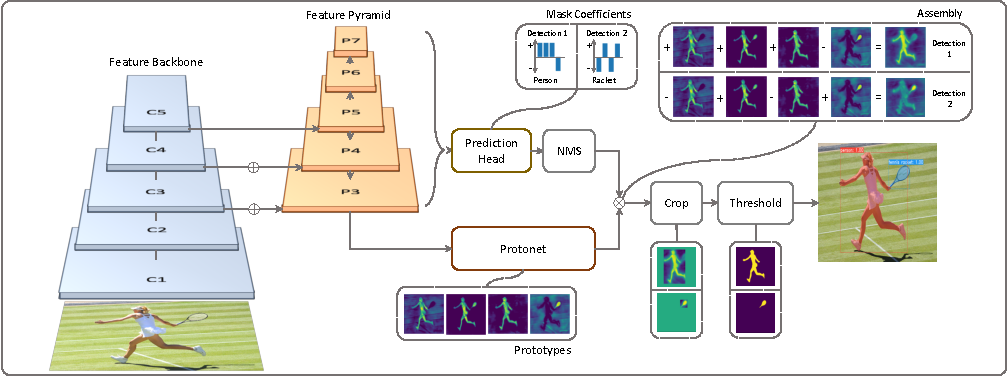
\includegraphics[width=\linewidth]{figures/yolact_fig_2-cropped}
    \caption{Figure~2 from \textit{YOLACT}. The figure shows how generated prototype masks are combined with instance-specific coefficients to produce the final instance masks.}
    \label{fig:yolact}
\end{figure}

\textit{YolactEdge} is a real-time instance segmentation method designed for edge devices, focusing on video processing.
Its functionality can be broken down into two main improvements over the original \textit{YOLACT} method:

\begin{enumerate}
    \item \textbf{\textit{TensorRT} Optimization:} \textit{YolactEdge} utilizes NVIDIA's \textit{TensorRT}~\cite{vanholder2016efficient} inference engine to optimize the neural network.\ \textit{TensorRT} provides mixed-precision support, optimal tensor layout, layer fusion, and kernel specializations.\ It quantizes model weights to \texttt{INT8} or \texttt{FP16} precision, which can speed up the processing while preserving accuracy.\ \textit{YolactEdge} explores the optimal mix between INT8 and FP16 weights for different model components, maximizing speed without significant degradation in accuracy.\ The \textit{TensorRT} optimization results in around a 4x improvement in speed when working with static images.
    \item \textbf{Exploiting Temporal Redundancy in Video:} \textit{YolactEdge} takes advantage of the temporal redundancy in videos, which means that neighboring frames in a video sequence are often highly correlated.\ Instead of computing expensive backbone features for every frame, YolactEdge divides the frames into two groups: keyframes and non-keyframes.\ For keyframes, the model computes all backbone and pyramid features.\ For non-keyframes, only a subset of features is computed, while the rest are transformed from the temporally closest previous keyframe.
\end{enumerate}

By combining \textit{TensorRT} optimization and exploiting temporal redundancy, YolactEdge can achieve real-time instance segmentation on edge devices such as Jetson AGX Xavier with a high frame rate and competitive accuracy.
This makes it an ideal solution for applications like robotics, autonomous driving, security, and augmented reality that require real-time processing and low latency.

\section{The YOLOv7 Instance Segmentation Model}
\label{sec:yolovseven}

\textit{YOLOv7}~\cite{wang2022yolov7}, as a state-of-the-art real-time object detection model, demonstrates significant quantitative improvements in object detection performance.
It not only excels in this primary task but also showcases its adaptability and effectiveness in related computer vision tasks, such as instance segmentation.

To achieve high-performance real-time instance segmentation, \textit{YOLOv7} is integrated with BlendMask, a technique introduced in the paper \enquote{BlendMask: Top-Down Meets Bottom-Up for Instance Segmentation}.
BlendMask builds upon the foundation laid by \textit{YOLACT}, but with a key difference in its approach to blending masks within bounding boxes.
While \textit{YOLACT} predicts a single scalar coefficient for each prototype mask, BlendMask predicts a low-resolution $(7*7)$ attention map for the same purpose, as described in Figure~\ref{fig:blendmask}.

\begin{figure}[htb]
    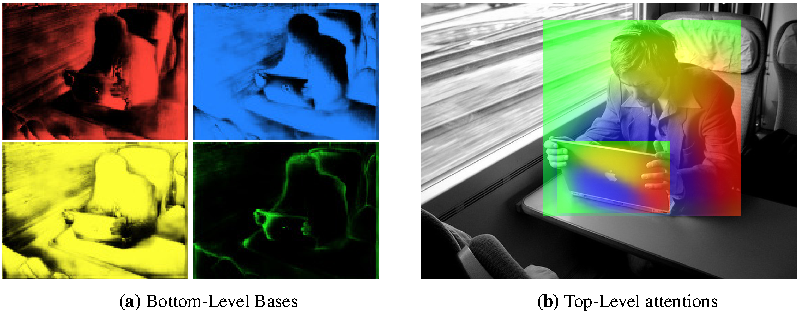
\includegraphics[width=\linewidth]{figures/blendmask_fig_3-cropped}
    \caption{Figure~3 from \textit{BlendMask}, showcasing how it replaces \textit{YOLACT's} Prototype Masks with Bottom-Level Bases which are combined using per-instance Top-Level Attention maps rather than coefficients.}
    \label{fig:blendmask}
\end{figure}

This attention map, which functions as a high-dimensional feature, is attached to each bounding box.
The blending of masks using the attention map results in a more precise and refined instance segmentation.
To leverage \textit{YOLOv7} for instance segmentation, the \textit{YOLOv7} object detection model is fine-tuned on the \textit{MS COCO}~\cite{lin2014microsoft} instance segmentation dataset.
The resulting \textit{YOLOv7}-mask model achieves a Mask AP (average precision) of $43.1\%$, while \textit{YOLACT} achieves a Mask AP of $35.4\%$ when using a \textit{ResNet-101} backbone.
The architecture of \textit{YOLOv7}-mask, as well as some of the qualitative corresponding results, are illustrated in Figure~\ref{fig:blendmask}.

% ----------------------------------------------------

\section{Map Data Formats}
\label{sec:opendrive}

This work depends on HD maps to inform viable heading choices for road user detections.
As map data formats for this task, both the \textit{OpenDRIVE}~\cite{dupuis2010opendrive, althoff2018automatic} and \textit{Lanelet2}~\cite{poggenhans2018lanelet2} map data formats are considered.
In both \textit{OpenDRIVE} and \textit{Lanelet2} formats, lane geometry representation is crucial for accurate road modeling and navigation.
\textit{OpenDRIVE} is an XML-based data format that describes road networks hierarchically.
It consists of roads, lanes, junctions, objects, and signals, with each road having a unique identifier and geometric information.
Lanes are classified into driving lanes, sidewalks, and shoulders, while junctions define connections between roads.
\textit{Lanelet2}, on the other hand, uses a combination of XML and OSM formats for data representation.
It is based on the concept of \enquote{lanelets}, which are individual driving lanes with associated traffic rules.
\textit{Lanelet2} includes left and right boundaries, regulatory elements, and routing graphs.

In \textit{OpenDRIVE}, lane geometry is represented using a combination of planar and lateral geometric information.
The geometry of a road is defined by a reference line, which is a parametric curve.
This curve is specified using a series of points and can be described by different types of geometry, such as straight lines, spirals, arcs, and clothoids.
The reference line represents the road's centerline, and the lanes are defined relative to it.
Lanes in \textit{OpenDRIVE} are divided into three categories: driving lanes, sidewalks, and shoulders.
Each lane has attributes such as width, type, and road marks.
The lateral position of a lane is described by a set of functions, which determine the lane's width as a function of its longitudinal position along the road.
This information, along with the road's reference line, is used to compute the geometry of individual lanes.

\textit{Lanelet2} uses a simpler approach for representing lane geometry.
It employs polygons, with each lanelet defined as a drivable polygon consisting of left and right boundaries.
The boundaries are sequences of nodes (points with longitude and latitude), which form linear or curved segments.
The nodes are ordered along the lanelet's direction, and the shape of the lanelet is derived by connecting corresponding nodes from the left and right boundaries.
Lane boundaries in \textit{Lanelet2} can be solid or dashed lines, indicating whether lane changes are allowed.
Unlike \textit{OpenDRIVE}, which uses parametric curves for defining road geometry, \textit{Lanelet2} uses a more straightforward representation based on sequences of points.
This approach can be less accurate in some cases, but it simplifies map data handling and provides better compatibility with OpenStreetMap data.

\begin{figure}[htb]
    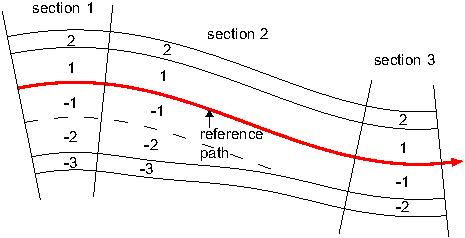
\includegraphics[width=0.49 \linewidth]{figures/opendrive_to_lanelet_fig_2_-cropped}
    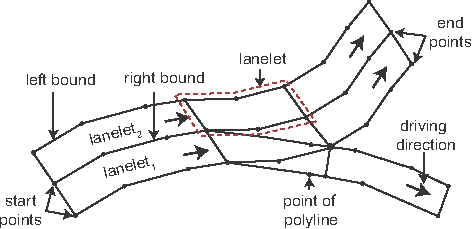
\includegraphics[width=0.49 \linewidth]{figures/opendrive_to_lanelet_fig_3-cropped}
    \caption{Figures~2 and~3 from~\cite{althoff2018automatic}. The left-hand-side image shows a typical \textit{OpenDRIVE}-based model with multiple lane-sections based on a common continuous reference line. The left-hand-side image shows the simpler modeling approach of \textit{Lanelet2}, where lanes are based on self-contained pre-triangulated shapes.}
    \label{fig:opendrive-lanlet}
\end{figure}

In summary, \textit{OpenDRIVE} represents lane geometry using parametric curves and a reference line, while \textit{Lanelet2} uses polygonal shapes defined by sequences of nodes.
\textit{OpenDRIVE} offers more accurate road geometry, but \textit{Lanelet2's} simpler representation can be easier to work with and integrate with other mapping data sources like OpenStreetMap.
This modeling difference is also highlighted in Figure~\ref{fig:opendrive-lanlet}.
In this work, we are compelled to use \textit{OpenDRIVE} as the input format for the HD map, as this format was used by Providentia's map data supplier.
However, the \textit{Lanelet2} format would be more suitable, as their approach to lane modeling is directly compatible with our heading interpolation algorithm, as described in Section~\ref{sec:hdmapgrids}.

% ----------------------------------------------------

\section{The Robot Operating System}
\label{sec:ros}

The \textit{Robot Operating System (ROS)}~\cite{quigley2009ros} is a flexible software framework for developing robotic applications.
Its main goal is to simplify the creation of complex and robust robot behavior across various platforms.

\textit{ROS} follows a graph architecture, where modular components called nodes communicate with one another through a publish-subscribe messaging model.
Nodes are single-purpose components responsible for specific tasks, such as controlling a sensor or processing data.
They exchange information by sending messages over named channels called \textit{topics}.
Another central component in \textit{ROS} is the Master, which manages the entire system by allowing nodes to find each other, register topics and services, and maintain a list of active nodes.

The framework provides several advantages for robotics applications, including hardware abstraction, low-level device control, efficient message passing, package management, and a rich ecosystem of tools and libraries.
These features make it easier for developers to build distributed robotics applications and promote modularity and code reusability.
In our case, we divide separate detector stages into different nodes, as described in Section~\ref{sec:arch}.

\section{SORT Object Tracking}
\label{sec:sort}

The \textit{Simple Online and Realtime Tracking (SORT)}~\cite{bewley2016simple} algorithm is an object tracking method that is specifically designed for tracking multiple objects in real-time.
It employs a combination of detection and tracking to maintain the identity of objects as they move across video frames.
\textit{SORT} is lightweight and computationally efficient, making it suitable for real-time applications.

At the core of the \textit{SORT} algorithm is the \textit{Kalman Filter}~\cite{welch1995kalman}, a recursive estimation technique that helps to predict the state of a dynamic system over time, even in the presence of noise.
In the context of object tracking, the \textit{Kalman Filter} is used to estimate the position, velocity, and other parameters of objects in the video frames.

Here is a step-by-step description of the \textit{SORT} algorithm and its use of \textit{Kalman Filters}:

\begin{enumerate}
    \item \textbf{Object Detection:} First, an object detection algorithm, such as YOLO (You Only Look Once) or Faster R-CNN, is applied to the input video frames to identify objects of interest and generate bounding box coordinates for each detected object.
    \item \textbf{Initialization:} For each detected object, a \textit{Kalman Filter} is initialized with the bounding box coordinates as the initial state.\ The state vector typically includes the position $(x, y)$ and velocity $(vx, vy)$ of the object's center.\ Additionally, a unique ID is assigned to each object.
    \item \textbf{Prediction:} For each object, the \textit{Kalman Filter} predicts its state in the next frame.\ This is done by applying a state transition model to the current state, which usually involves updating the position based on the velocity.
    \item \textbf{Data Association:} In the subsequent frame, the newly detected objects are matched with the predicted states of the existing tracked objects.\ This association is achieved using a distance metric, typically the Intersection over Union (IoU) or the Mahalanobis distance.\ A bipartite graph matching algorithm, such as the Hungarian algorithm~\cite{kuhn1955hungarian}, is employed to find the optimal assignment between detections and tracked objects.
    \item \textbf{Update:} Once the data association is completed, the \textit{Kalman Filter} is updated with the new measurements (bounding box coordinates) of the associated detected objects.\ This step incorporates the new observations into the existing state estimate, considering both the prediction and the measurement uncertainties.
    \item \textbf{Handling Occlusions and New Objects:} If a tracked object is not detected in the new frame, its \textit{Kalman Filter's} state is still updated based on the prediction alone.\ If an object is missing for a certain number of consecutive frames, it is removed from the tracking list.\ Conversely, if a new object is detected, a new \textit{Kalman Filter} is initialized and added to the tracking list.
    \item \textbf{Output:} The final output of the \textit{SORT} algorithm is a list of tracked objects, each with a unique ID and an updated bounding box for each frame.
\end{enumerate}

In summary, the \textit{SORT} algorithm uses \textit{Kalman Filters} to predict and update the state of objects in a video sequence, maintaining their identities while tracking their positions and velocities over time.\ The data association step ensures that the correct detections are matched with the corresponding tracked objects, making the tracking robust and efficient.

% ----------------------------------------------------

\section{The DBSCAN Algorithm}
\label{sec:dbscan}

\textit{DBSCAN}, which stands for \textit{Density-Based Spatial Clustering of Applications with Noise}~\cite{schubert2017dbscan}, is a popular unsupervised machine learning algorithm designed for cluster analysis.
It works by identifying dense regions in the input data, separating them into distinct clusters, and treating low-density regions as noise.

\textit{DBSCAN} has the following key functionalities:

\begin{enumerate}
    \item \textbf{Density-based clustering:} The algorithm groups data points based on their density in the feature space.\ A dense region is defined as an area with a high concentration of data points, while a low-density region has fewer data points.
    \item \textbf{Automatic detection of the number of clusters:} Unlike some other clustering algorithms, like K-means, \textit{DBSCAN} does not require the user to specify the number of clusters beforehand.\ The algorithm automatically determines the number of clusters based on the input data.
    \item \textbf{Robustness to noise:} \textit{DBSCAN} can identify and separate noise from the data.\ Noise is defined as data points that do not belong to any dense region and are not part of any cluster.
    \item \textbf{Handling arbitrary shapes:} \textit{DBSCAN} can identify and create clusters with varying shapes and sizes, unlike some other clustering algorithms that assume clusters have a spherical or circular shape.
\end{enumerate}

The \textit{DBSCAN} algorithm works in the following steps:

\begin{enumerate}
    \item \textbf{Initialize:} Two main parameters need to be defined: $\epsilon$, which is the radius around a data point, and $N_\text{min}$, the minimum number of data points required to form a dense region.
    \item \textbf{Iterate through the data points:} For each unvisited data point in the dataset, perform the following steps:
    \subitem Mark the current data point as visited.
    \subitem Find all neighboring data points within the $\epsilon$ radius.
    \subitem If the number of neighbors is greater than or equal to $N_\text{min}$, mark the current data point as a core point and create a new cluster.\ Recursively add all the connected neighbors (directly or indirectly) to the cluster using a depth-first search approach.
    \subitem If the number of neighbors is less than $N_\text{min}$, mark the current data point as noise.
    \item \textbf{Cluster assignment:} Assign data points to their respective clusters.\ Core points are assigned to a specific cluster, border points are assigned to the nearest core point's cluster, and noise points are not assigned to any cluster.
\end{enumerate}

The \textit{DBSCAN} algorithm is particularly useful for datasets with spatial or geographical data, as well as for datasets with complex structures and noise.
In the case of this work, the \textit{DBSCAN} algorithm is applied to denoise vehicle bottom contours which have been projected out from the vehicle's instance mask into $3D$ space.
This is further explained in Section~\ref{sec:botcont}.

% ----------------------------------------------------

\section{The L-Shape Fitting Algorithm}
\label{sec:lshapefitting}

The \textit{L-Shape-Fitting} algorithm is used to find the best-fitting rectangle for a segmented cluster of points.
The algorithm assumes that the vehicle being tracked can be approximated by an L-Shape rectangle model, which consists of two perpendicular lines that intersect at a corner.
The goal is to find the optimal disjunction of the $m$ points into two sets ($P$ and $Q$) and the optimal parameters ($\theta$, $c_1$, $c_2$) for the two perpendicular lines corresponding to the points in $P$ and $Q$, respectively.

\begin{figure}[htb]
    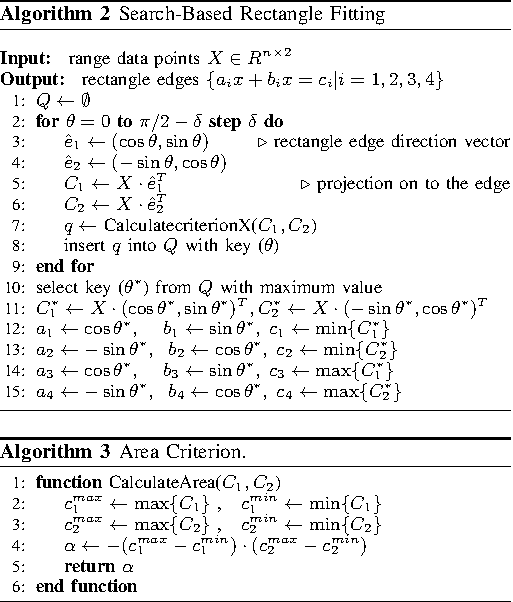
\includegraphics[width=0.49\linewidth]{figures/l_shape_fitting_fig_algs_1-cropped}
    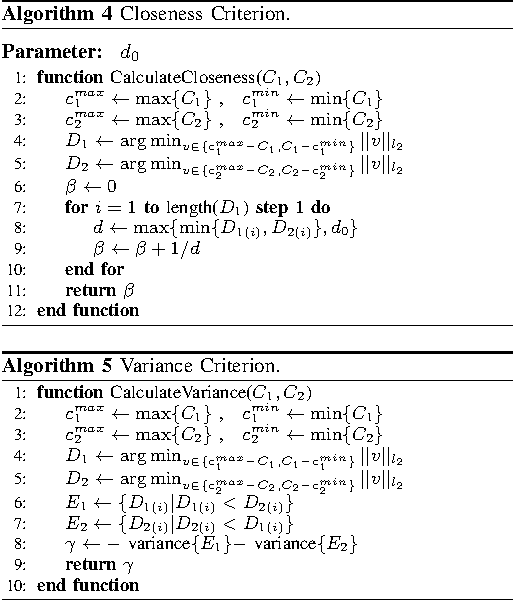
\includegraphics[width=0.49\linewidth]{figures/l_shape_fitting_fig_algs_2-cropped}
    \caption{Algorithms~2-5 from \textit{L-Shape-Fitting}~\cite{zhang2017efficient}. Algorithm~2 shows the main theta search loop, while Algorithms~3-5 are possible implementations of the \texttt{CalculateCriterionX} function.}
    \label{fig:lsf-algs}
\end{figure}

The algorithm uses a search-based approach (see Algorithm~2 of Figure~\ref{fig:lsf-algs}) to find the best-fit rectangle approximately.
It iterates through all possible directions of the rectangle and for each direction, it calculates the distances of all the points to the rectangle's four edges.
Based on these distances, the points are split into $P$ and $Q$, and the corresponding errors are calculated as the objective function.
After iterating through all directions, the algorithm selects the optimal direction which achieves the smallest error, and fits the rectangle based on that direction.

The algorithm offers three different criteria for selecting the best-fitting rectangle: rectangle area minimization, points-to-edges closeness maximization, and points-to-edges squared error minimization.
Each criterion can be chosen to play the role of the \texttt{CalculateCriterionX} function in the algorithm provided in Figure~\ref{fig:lsf-algs}.
The choice of criterion depends on the specific requirements of the application.

The experimental results show that the algorithm is highly accurate and efficient, with a small mean and standard deviation of the estimation error.
Albeit computationally the most expensive, the variance criterion achieves the highest correctness, while the area minimization criterion sometimes fails to estimate the correct heading.

However, the algorithm may not always achieve perfect results.
For instance, the algorithm may fail to estimate the correct heading if the scan points are too sparse, or if there are points outside or inside of the L-Shape model.
This is where the previously mentioned (see Section~\ref{sec:dbscan}) \textit{DBSCAN}~\cite{schubert2017dbscan} algorithm comes in to denoise the bottom contour points.
Nevertheless, the impact of such imperfect cases on vehicle tracking can be minimized by biasing the algorithm's search space towards correct solutions using tracking and the HD map, as is done in this work.

% ----------------------------------------------------

\section{Evaluation Metrics}
\label{sec:evalmetrics}

Like in 2D object detection, the \textit{Average Precision (AP)} is also used as the main evaluation metric in 3D object detection.
The predictions are first assigned to their corresponding ground truths according to a specific similarity measure to compute AP\@.
The most used similarity measure is the \textit{Intersection over Union (IoU)}, which is the geometric overlap between the ground truth 3D bounding box A and the estimated 3D bounding box B\@.
IoU is defined like this:

\[
\text{IoU}(A,B) = \frac{|A \cap B|}{|A \cup B|}
\]

The \textit{IoU} measure is used to judge a matched prediction as a \textit{True Positive (TP)} or a \textit{False Positive (FP)} by comparing it with a certain threshold.
Then, the recall $r$ and precision $p$ can be computed from the ranked detection results according to the following (FN denotes False Negatives):

\[
    r = \frac{\text{TP}}{\text{TP}+\text{FN}}, p = \frac{\text{TP}}{\text{TP}+\text{FP}}
\]

The precision can be regarded as a function of recall, i.e., $p(r)$: As recall approaches zero, the precision will rise, as there are fewer and fewer False Positives in the denominator.
Conversely, a rising recall is usually associated with a drop in precision, as the reduced number of False Negatives leads to new False Positives.
The interpolated precision values across a range of recall values is defined as AP:

\[
    \text{AP} = \frac{1}{\mathbb{R}} \sum_{r \in \mathbb{R}} p(r)
\]

where the set $\mathbb{R}$ refers to a discrete set of values in practice.
The mean of this value across all object classes is called $mAP$.
The AP metric is commonly used to evaluate object detection performance, but it only considers the localization of objects and does not account for other factors such as dimension and orientation.
To address this limitation, \textit{nuScenes}~\cite{caesar2020nuscenes} proposed a set of True Positive (TP) metrics that measure other prediction errors from the true positives.

The five TP metrics are defined as positive scalars, including the \textit{Average Translation Error (ATE)}, \textit{Average Scale Error (ASE)}, \textit{Average Orientation Error (AOE)}, \textit{Average Velocity Error (AVE)}, and \textit{Average Attribute Error (AAE)}.
The \textit{ATE} measures the Euclidean distance between the object center on the 2D ground plane in meters.
The \textit{ASE} is the 3D Intersection over Union (IoU) error after aligning orientation and translation.
The \textit{AOE} is the smallest yaw angle difference between the predictions and ground truths in radians.
The \textit{AVE} is the absolute velocity error as the L2 norm of the velocity differences in 2D in meters per second.
Finally, the \textit{AAE} is defined as 1 minus attribute classification accuracy $(1-acc)$.

To obtain a single scalar score, \textit{nuScenes}~\cite{caesar2020nuscenes} computes the mean TP metric (mTP) over all object categories $\mathbb{C}$ for each TP metric using the following equation:

\[
    \text{mTP}_k = \frac{1}{\mathbb{C}} \sum_{c \in \mathbb{C}} \text{TP}_{k,c}
\]

where $\text{TP}_{k,c}$ denotes the k-th TP metric (e.g., $k=1$ means the ATE) for category $c$.
To integrate all the mentioned metrics into a scalar score, \textit{nuScenes} proposes the \textit{nuScenes} Detection Score (NDS) equation that combines the mAP and mTPk scores.
The NDS is calculated using the following equation:

\[
    \text{NDS} = \frac{1}{10} \left[5 * \text{AP} + \sum^5_{k=1}(1-\text{min}(1, \text{mTP}_k))\right]
\]

where AP is the mean average precision defined previously.
The term $1-\text{min}(1, \text{mTP}_k)$ is used to ensure that each TP metric contributes to the score positively, and the division by 10 is used to ensure that the score is in the range $[0, 1]$.

% ----------------------------------------------------

% !TeX spellcheck = en_US

\chapter{System Design}
\label{ch:system}

\section{Distributed Architecture}
\label{sec:arch}

Pub-Sub Nodes

% ----------------------------------------------------

\section{The 2D Object Detector}
\label{sec:segmentation}

2D Detector \par
Downscaling \par
Connection to Cameras \par
Communication - Bit Packing

\section{The 3D Object Detector}
\label{sec:mono3doverview}

Mono3D Overview Diagram

% ----------------------------------------------------

\section{Bottom Contour Extraction and Filtering}
\label{sec:botcont}

Bottom Contour Extraction \par
Projection \par
Filtering

\section{Detection of Vulnerable Road Users}
\label{sec:pedcyc}

Worth improving

\section{Bottom Contour L-Shape Fitting}
\label{sec:botcontlsf}

Bottom Contour L-Shape Fitting

% ----------------------------------------------------

\section{HD Map Lookup Grids}
\label{sec:hdmapgrids}

HD Map Grids \par
Rendering \par
Resolution

% ----------------------------------------------------

\section{HD-Map-Augmented L-Shape Fitting}
\label{sec:hdmaplsf}

HD Map Grid Lookup - Early \par
Yaw Lookup Histogram \par
Confidence

% ----------------------------------------------------

\section{Tracking-Augmented L-Shape Fitting}
\label{sec:trackinglsf}

Historical Plausibility \par
2D Tracking SORT Lookup

% ----------------------------------------------------

\section{Joint Height and Position Estimation}
\label{sec:size}

L/W/H Dimension Filtering \par
Height Estimation

% ----------------------------------------------------

\section{Late HD Map Lookup}
\label{sec:hdmaplate}

HD Map Grid Lookup - Late \par
Tempting, Simple, Bad

% ----------------------------------------------------

\section{3D Tracking}
\label{sec:trackthreed}

3D Tracking \par
LIDAR Label Shifting

% !TeX spellcheck = en_US

\chapter{Evaluation}


% !TeX spellcheck = en_US

\chapter{Conclusion}
\label{ch:conclusion}

In the previous chapter, we evaluated various aspects of our proposed two-stage monocular infrastructure traffic object detection architecture, \textit{MonoDet3d}.
We analyzed the performance of different models on the \textit{Providentia Intersection Scenario} dataset, using both detailed object categories and the vehicle super-category.
Focusing on vehicles, the best model for the \texttt{S110-S1} perspective achieves a score of $55.60\%$ ($65.54\%$ mAP), while for the \texttt{S110-S2} perspective, the best model scores $50.90\%$ ($60.69\%$ mAP).
The best model across all object categories and scenes exhibits a score of $40.29\%$ ($38.94\%$ mAP).

Moreover, we provided a thorough ablation study of the architecture across all possible configuration regimes.
This covered the impact of different L-Shape-Fitting augmentations, bottom-contour/size filters, different instance segmentation models, and various filter types.
We also accounted for the synchronization lag between the camera frames and the LiDAR-sensor-based labels.

Despite the comprehensive evaluation, there are some shortcomings that can be addressed.
Firstly, the early version of the \textit{A9R1} dataset used in the evaluation has some issues, as some LiDAR labels are inaccurate, potentially affecting the model performance assessment.
This might also explain the ceiling of $~40\%$ IoU, which we seemingly cannot overcome.
Secondly, ablation studies for the VRU detection algorithm and the position-height regression algorithm are missing, which could provide more valuable insights into the system's performance and help identify areas for improvement.

In summary, our evaluation offers a thorough understanding of the system's performance, its limitations, and the challenges that arise from different camera perspectives and computational constraints.
It may now be concluded without a doubt, that the HD map as an auxiliary bias for the L-Shape-Fitting algorithm offers a very significant improvement, guiding the proposed architecture into the realm of production-readiness.
Without the HD map, the detector does not reach an acceptable orientation error.
Therefore, the research hypothesis is confirmed insofar as concluding, that tracking alone does not substitute the HD map as a bias for deciding vehicle orientations.
However, additional analysis and improvements can be made by addressing the mentioned shortcomings, to ultimately enhance the system's performance and reliability even further.

\par\vspace*{\fill}
\epigraph{``Begin at the beginning," the King said gravely, ``and go on till you come to the end: then stop."}{--- \textup{Lewis Carroll}, Alice in Wonderland}

% !TeX spellcheck = en_US

\chapter{Future Work}
\label{ch:future}

In this chapter, we outline potential avenues for future work to further enhance the performance, capabilities, and robustness of our traffic object detection and segmentation system.

\section{Improved Non-Maximum Suppression (NMS)}
\label{sec:nms}

A common issue encountered in our system is the overlapping of bounding boxes, particularly for pedestrians inside bicycles or vans inside trucks.
To address this problem, we can explore more advanced non-maximum suppression (NMS) techniques that better handle these cases and suppress overlapping boxes, thus improving the system's overall accuracy and robustness.

\section{Substituting HD Maps}
\label{sec:nomap}

Instead of relying solely on HD maps for obtaining heading information, we can explore deriving this information directly from the optical flow.
This approach could offer a more adaptive and flexible solution to changing environments and potentially improve the system's performance in situations where the HD maps are unavailable or inaccurate.

\section{Extended use of Kalman Filters}
\label{sec:extkalman}

The current implementation of Kalman filters in our system does not include heading information in the state.
This omission renders the current approach non-viable for accurate tracking and prediction de-noising.
Extending the Kalman filter to include heading information would significantly improve its effectiveness in estimating the state of the tracked objects.

\section{Improving Pedestrian/Cyclist Detection}
\label{sec:improvepedcyclist}

The current solution for pedestrian and cyclist (VRU) detection is highly unoptimized, as the focus of this work was mostly directed towards road vehicle pose estimation.
Future work should focus on optimizing and refining the detection algorithm, increasing its accuracy and robustness, and also attempting to predict VRU orientations.

\section{Neural Keypoint Estimation}
\label{sec:neuralkeypoints}

The long tail robustness of our system can be improved by incorporating neural keypoint estimation techniques.
This approach would help better handle obstructions, occlusions, and unusual vehicle orientations, ultimately enhancing the system's performance in complex and dynamic traffic scenarios.
It could also unify the VRU/Vehicle detection pipelines, and further improve the system's runtime performance.
This presents itself as a very promising research direction.

\section{Amodal Instance Segmentation}
\label{sec:amodal}

Amodal instance segmentation is a way if predicting instance masks while also completing masks where the detection is cut off or obstructed.
This may be a viable alternative to keypoints for object detection and segmentation, as it woul be a less intrusive architectural change.
While it may not be as robust as keypoints in some cases, it might still present a valid approach to improve our system's overall performance.
By investigating amodal instance segmentation techniques, we can potentially enhance the system's ability to detect and segment objects in challenging traffic scenarios.

\par\vspace*{\fill}
\epigraph{``Optimism is a strategy for making a better future. Because unless you believe that the future can be better, you are unlikely to step up and take responsibility for making it so."}{--- \textup{Noam Chomsky}}

%% !TeX spellcheck = en_US
\chapter{About TUMlatex}%

\section{Introduction}
This TUMlatex project represents a cooperation of several chairs of the Technical University of Munich to provide a compact and easy-to-use LaTeX package for both, employees and students.

If you are interested in using this package, please read Section~\ref{quick-start-guide}.

If you are an advanced LaTeX user and want to contribute to this project, please read Section~\ref{guide-for-developers}.

If you are responsible for the LaTeX templates of your chair and you are interested in joining this collaboration, please contact the current maintainer Michael Kreutz (\href{mailto:m.kreutz@tum.de}{m.kreutz@tum.de}).

\section{Quick-Start-Guide for Beginners}\label{quick-start-guide}
This project aims to provide an easy-to-use solution for unexperienced or even first-time LaTeX users. As a first step, please read the installation instructions of Section~\ref{installation}.

\subsection{Installation}\label{installation}

If you are using TUMlatex for the first time, please pass through the following steps carefully.

\subsubsection{Setup your LaTeX Environment}\label{setup-environment}

First of all you have to install a LaTeX environment on your PC.
You may skip this step, if you are using a PC of the university with a pre-installed LaTeX environment (e.g. TUM-PC).

\begin{itemize}
    \item For \textbf{Windows} users: Please install the newest version of \underline{\href{https://miktex.org/howto/install-miktex}{MiKTeX}} (see below for full installation).
    \item For \textbf{Mac} users: Please install the newest version of \underline{\href{https://www.tug.org/mactex/}{MacTeX}} (see below for full installation).
    \item For \textbf{Linux} (Ubuntu, \underline{\href{https://www.tug.org/texlive/}{TeXLive}}) - Option A (outdated version - not recommended): Install the default packages texlive-full and biber via apt-get shipped with your Ubuntu distribution.
    \item For \textbf{Linux} (Ubuntu, \underline{\href{https://www.tug.org/texlive/}{TeXLive}}) - Option B (\textbf{newest version - recommended}): Download the TUMlatex package of your chair (see Section~\ref{get-tumlatex}), unzip it and run the automatic installer script \code{UbuntuInstallTexliveNewest.sh} as root\\(\code{sudo ./UbuntuInstallTexliveNewest.sh}) located in XXXTools (replace XXX by your chair abbreviation).
\end{itemize}

\textit{Note: Without any warranty you may use a different LaTeX environment.}

\vspace{0.3cm}

\textbf{Important:} If the amount of free memory on your PC permits, be sure to install all packages.
Otherwise it is likely, that you are missing some necessary packages and have to install them on your own.

\begin{itemize}
    \item For \textbf{Windows} users: Install all packages via the \underline{\href{https://docs.miktex.org/2.9/manual/pkgmgt.html}{MiKTeX Package Manager}}.
    \item For \textbf{Mac} users: Install the \underline{\href{http://www.tug.org/mactex/mactex-download.html}{Full MacTeX package}}.
    \item For \textbf{Linux} users: Both options (A and B) mentioned above will install a full installation of TeXLive.
\end{itemize}

\subsubsection{Optional: Update your LaTeX Environment}

In some cases this is necessary in order to avoid compilation errors due to outdated standard packages. Again you may skip this step if this is not your private PC.

\begin{itemize}
    \item For Windows users: Please follow \underline{\href{https://miktex.org/howto/update-miktex}{this guide}}.
    \item For Mac users: You can use the graphical updating tool \underline{\href{http://amaxwell.github.io/tlutility/}{TeX Live Utility}} to update your packages.
    \item For Linux users: If you chose option B (see Section~\ref{setup-environment}) open a terminal and update the TeXLive package manager and all packages with the command \code{sudo tlmgr update --self --all --reinstall-forcibly-removed}
\end{itemize}

\subsubsection{Setup your LaTeX Editor}

You can use any editor you like. However, the open-source and cross-platform LaTeX editor \underline{\href{http://www.texstudio.org/}{TeXstudio}} is recommended. In this case you can use the \textbf{auto-completion feature} by copying the provided syntax file (\code{.cwl-file}, shipped within the \code{.zip} file, see Section~\ref{get-tumlatex}) to the folder

\begin{itemize}
    \item \code{\%APPDATA\%\textbackslash Roaming\textbackslash texstudio\textbackslash completion\textbackslash user} for Windows users or equivalently
    \item \code{$\sim$/.config/texstudio/} for Linux or Mac users.
\end{itemize}

Furthermore you may enable the shell-escape option of pdflatex (optional, but neccessary for tikz-externalize to work):

\begin{enumerate}
    \item Navigate to \textit{Options $\rightarrow$ Configure TeXstudio $\rightarrow$ Commands}
    \item Change \textit{PdfLaTeX} to \code{pdflatex -synctex=1 -shell-escape -interaction=nonstopmode \%.tex}
\end{enumerate}


You also should change the default bibliography tool from \textit{bibtex} to \textbf{\textit{biber}}:

\begin{enumerate}
    \item Navigate to \textit{Options $\rightarrow$ Configure TeXstudio $\rightarrow$ Build}
    \item Change \textit{Default Bibliography Tool} to \code{txs:///biber}
\end{enumerate}


\textit{Note: You can also use bibtex as bibliography backend with the TUMlatex packages. However, you have to pass \code{optBibtex} instead of \code{optBiber} to the package. Furthermore some commands related to the bibliography are different (ask Google for help).}

\subsubsection{Get the latest Release of the TUMlatex Package}\label{get-tumlatex}

If you are reading this document you probably already have downloaded the TUMlatex package.
However, it is recommended to check if you are using the latest version.
In the following table you find the chair-related TUMlatex packages:

\begin{table}[h]
    \centering
    \begin{tabular}{lll}
        \toprule
        Dept. & Chair & TUMlatex Package \\
        \midrule
        MW & Aerodynamics and Fluid Mechanics & \underline{\href{https://gitlab.lrz.de/AM/TUMlatex/-/jobs/artifacts/release/download?job=ReleaseMWAER}{AERlatex.zip}} \\
        MW & Applied Mechanics & \underline{\href{https://gitlab.lrz.de/AM/TUMlatex/-/jobs/artifacts/release/download?job=ReleaseMWAM}{AMlatex.zip}} \\
        MW & Automotive Technology & \underline{\href{https://wiki.tum.de/display/ftm/Latex-Vorlage}{FTMlatex}} \\
        MW & Machine Tools and Industrial Management & \underline{\href{https://gitlab.lrz.de/AM/TUMlatex/-/jobs/artifacts/release/download?job=ReleaseMWIWB}{IWBlatex.zip}} \\
        MW & Central Teaching Unit & \underline{\href{https://gitlab.lrz.de/AM/TUMlatex/-/jobs/artifacts/release/download?job=ReleaseMWZL}{ZLlatex.zip}} \\
        IN & I6 - Robotics, AI \& Embedded Systems & \underline{\href{https://gitlab.lrz.de/AM/TUMlatex/-/jobs/artifacts/release/download?job=ReleaseINRAI}{RAIlatex.zip}} \\
        \bottomrule
    \end{tabular}
\end{table}

The packages include (replace "\code{XXX}" by your chair abbreviation)

\begin{itemize}
    \item the main class file \code{XXXlatex.cls},
    \item the main package file \code{XXXlatex.sty}
    (This is an alternative to using the main class file.
    This is helpful, if you write a paper and have to use the baseclass provided by the publisher),
    \item the syntax file \code{XXXlatex.cwl} for auto-completion in \underline{\href{http://www.texstudio.org/}{TeXstudio}},
    \item a license file \code{XXXlatex\_LICENSE.txt} containing licensing information,
    \item a folder \code{XXXDocumentation} containing the package documentation (therein precompiled as \code{main.pdf}),
    \item a folder \code{XXXTemplates} containing a selection of useful templates which you can copy and directly use.
    \item a folder \code{XXXTools} containing a selection of useful tools (e.g. TeXLive setup script).
\end{itemize}


\subsection{Create your own Document}

The \textbf{recommended way} to create a new document is to
\begin{enumerate}
    \item select an appropriate template in the template folder \code{XXXTemplates},
    \item \textbf{copy the whole template folder} (e.g. \code{XXXDocument}) wherever you want,
    \item open the \code{main.tex} file in the template folder with your favorite LaTeX-editor,
    \item initially compile it (using \textit{pdflatex} and optionally \textit{biber/bibtex}) and check for errors,
    \item make your changes and fill it with content and
    \item compile it (using \textit{pdflatex} and optionally \textit{biber/bibtex}).
\end{enumerate}

\textit{
    Note: As an alternative way it is possible to use the main class (\code{.cls}-file) or the main package (\code{.sty}-file) as a shared resource by copying it to your local \code{texmf} folder.
    However, in this case you may not be able to compile old documents, which have been created with a different version of this package.
    Thus it is \textbf{strongly recommended} to make a copy of the main class file (\code{XXXlatex.cls}) for each of your documents!
}

\subsection{Documentation}

The documentation of the packages is included in the folder \code{XXXDocumentation} (precompiled as file \code{main.pdf}).
Feel free to have a look at the source code of the documentation, in order to learn how to do stuff.
Be aware that most of the source code is automatically generated.

\subsection{Bugs, Errors and Suggestions}\label{bugs-errors-suggestions}

If you recognize any bug/error or you have a suggestion to make this package (even) better, please feel free to open an \underline{\href{https://gitlab.lrz.de/AM/TUMlatex/issues}{Issue}}.

\textbf{Important:} Assign the corresponding maintainer of your chair to the issue (see \underline{\href{https://gitlab.lrz.de/AM/TUMlatex}{LRZ GitLab}}).
Expect no support for unassigned issues - they will be deleted immediately!

Please use the default \textbf{Labels} to categorize your issue. Please also provide additional information like your
\begin{itemize}
    \item operating system (+ version),
    \item LaTeX environment (+ version) and
    \item LaTeX editor and (+ version).
\end{itemize}


\section{Guide for Developers/Contributors}\label{guide-for-developers}

For information on how to contribute to this project please have a look at the \underline{\href{https://gitlab.lrz.de/AM/TUMlatex/blob/develop/CONTRIBUTING.md}{Contribution Guide}}.

\section{Support}

For support, please directly contact the responsible package maintainer of you chair (see "maintainer" in Section~\ref{bugs-errors-suggestions}).

\textbf{Important:} If your are not associated with a chair or your chair is not part of the TUMlatex project, please read following note:
\textit{
    We are happy that you use TUMlatex and that you appreciate our effort in making a good LaTeX template for TUM members.
    However, please understand that this project is maintained by various PhD students, who contribute to the template mainly in their spare time (actually we do not get paid for this - its our personal commitment).
    Thus, we limit our "support" to employees and students of our associated chairs.
    Certainly, we are happy for any bug report, however, we can not assist everybody in using this template neither can we respond to individual feature requests.
    We hope you can understand this.
}

\section {License Notes}

Copyright (c) 2021 Technical University of Munich (\url{https://www.tum.de/})

This work may be distributed and/or modified under the conditions of the LaTeX Project Public License, either version 1.3 of this license or (at your option) any later version.
The latest version of this license is in \url{http://www.latex-project.org/lppl.txt} and version 1.3 or later is part of all distributions of LaTeX version 2005/12/01 or later.

This work has the LPPL maintenance status 'maintained'.
The current maintainer of this work is Michael Kreutz (\href{mailto:m.kreutz@tum.de}{m.kreutz@tum.de}).

This work consists of all files of the GitLab repository \url{https://gitlab.lrz.de/AM/TUMlatex}.
%
%
%% !TeX spellcheck = en_US
\chapter{I6 Submission Guidelines}%

This chapter gives an overview about the expected format of a thesis at the Chair of Robotics, Artificial Intelligence and Real-time systems.
It mostly focuses on the format on your written thesis.
For a general overview of the submission guideline please refer to the  \underline{\href{https://wiki.tum.de/display/I6intern/Thesis+Submission+Guidelines}{I6 Wiki}}.

When writing your thesis please use the \code{RAIStudentThesis} template.
It should be in line with the IN TUM thesis guidelines (last checked: 08/02/2020).
However, please always reassure that this is still the case. In other subjects, please make sure that the format meets your individual requirements.
When handing it in, please include an additional copy for your advisor. Moreover make sure your that thesis fulfills the following requirements.

\section{Citations}

We recommend that you use \href{https://ctan.org/texarchive/bibliography/bibtex/contrib/german/din1505}{\code{alphadin}} citation style when working with bibtex, or \code{alpha} when using biblatex/biber. Your bibliography should look like this:

\begin{table}[htb]
    \begin{tabular}{lp{13.5cm}}
        $[$BM92$]$ & Besl, P. J. and McKay, N. D. “Method for registration of 3-D shapes”. In: Sensor
        fusion IV: control paradigms and data structures. Vol. 1611. International Society
        for Optics and Photonics. 1992, pp. 586–606.\\
        $[$CM92$]$ & Chen, Y. and Medioni, G. “Object modelling by registration of multiple range
        images”. In: Image and vision computing 10.3 (1992), pp. 145–155.\\
    \end{tabular}
\end{table}

When quoting an author word-by-word please include a page number in the reference.

\section{Figures}

Please use vector graphics when including figures or diagrams in your thesis.
If you create them with \href{https://en.wikipedia.org/wiki/PGF/TikZ}{PGF/TIKZ} or \href{https://inkscape.org/}{Inkscape} it also possible to add texts directly from Latex to ensure a consistent typesetting.
There is an unwritten rule, saying figures not referenced in your text are unnecessary.

When citing a figure include the reference in the figure's label (including the page number).

\section{Math Notation}

When using formulas or pseudocode use the following notation style:

\begin{table}[htb]
    \begin{tabular}{p{2.9cm}lp{5.1cm}p{3.8cm}}
        \toprule
        \textbf{Type} & \textbf{Example} & \textbf{Code (Math Mode)} & \textbf{Comment} \\
        \midrule

        \multicolumn{4}{l}{\textbf{General items}} \\
        \midrule
        Scalars	& $a$ & \code{a} & lower case, italic \\
        Functions & $\textrm{sin}(x)$ & \code{\textbackslash textrm{sin}(x)} & regular text \\
        Units & 42\,Hz & \code{42\textbackslash,\textbackslash textrm{Hz}} & half-space between number and unit; unit in regular text \\
        Angles & $\alpha$ & \code{\textbackslash alpha} & Greek letters \\
        Absolute value & $\mid a \mid$ & \code{\textbackslash mid a \textbackslash mid} \\
        Modulo & mod & \code{\textbackslash textrm\{mod\}} \\
        \midrule
        \multicolumn{4}{l}{\textbf{Vectors and matrices}}\\
        \midrule
        Vectors	& $\boldsymbol{v}$ & \code{\textbackslash boldsymbol\{v\}} & lower case, italic, bold \\
        Matrices & $\boldsymbol{M}$ & \code{\textbackslash boldsymbol\{M\}} & upper case, italic, bold \\
        Variable indices & $\boldsymbol{x}_i$ & \code{\textbackslash boldsymbol\{x\}\_i} \\
        Static indices & $\boldsymbol{x}_\textrm{min}$ & \code{\textbackslash boldsymbol\{x\}\_\textbackslash textrm\{min\}} \\
        Unit vectors & $\textbf{e}_x$ & \code{\textbackslash textbf\{e\}\_x} \\
        Identity matrices & $\textbf{Id}_n$ & \code{\textbackslash textbf\{Id\}\_n}	\\
        Transpose & $\boldsymbol{x}^\textrm{T}$ & \code{\textbackslash boldsymbol\{x\}\^{}\textbackslash textrm\{T\} } & T in superscript and regular font \\
        Vector product (cross product) & $\times$ & \code{\textbackslash times} \\
        Dot product	& $\cdot$ & \code{\textbackslash cdot} \\
        \midrule
        \multicolumn{4}{l}{\textbf{Sets and sequences}}\\
        \midrule
        Sets & $A = \{ 1, 2, 3 \}$ & \code{A = \textbackslash \{ 1, 2, 3 \textbackslash \}} & upper case, italic \\
        Sequence & $\mathcal{A} = \langle 1,2,3 \rangle$ & \code{\textbackslash mathcal\{A\} = \textbackslash langle 1,2,3 \textbackslash rangle} \\
        Set without	& $A \backslash \{ e \}$ & \code{A \textbackslash backslash \textbackslash \{ e \textbackslash \}} \\
        Unification	& $A \cup \{ e \}$ & \code{A \textbackslash cup \textbackslash \{ e \textbackslash \}} & \\

        \bottomrule
    \end{tabular}
\end{table}

Always use single letters for variable names.

\section{Length}

Stundents often ask for a required number of pages.
However, there are no fixed page limits or requirements for bachelor's or master's theses.
As a point of reference, most bachelor's have around 40 to 60 pages and while master's thesis usually reach 60 to 80 pages (including abstract, table-of-contents, lists of figures, lists of tables and bibliography).
If your thesis is going to be longer than 100 pages, your advisor and/or supervisor will most likely not read all of it.
Detailed information can be found in your module handbook (see \url{campus.tum.de}).

\section{Cover}

The main directory of the \code{RAIStudentThesis} template contains two \code{*.tex}: \code{main.tex} and \code{cover.tex}.
Start by using \code{main.tex} to write your thesis.
Once you have completed your work and you know how large the spine of the book will be you can use \code{cover.tex} to generate a matching cover for your printed copies.

\section{CD or DVD}

\textbf{Note:} A CD or DVD is not required for the official copy you submit to the faculty or your program coordinator.
If in doubt check your program's website!

\vspace{0.5cm}

For your advisor's/ supervisor's copy of your thesis please add a CD or DVD on the last inner page of your thesis including:

\begin{enumerate}
    \item A digital copy of your thesis (including its Latex sources)
    \item The code you programmed
    \item The dataset(s) you used for your evaluation results
\end{enumerate}

As a rule of thumb, the disk should include everything required to reproduce your results.
%
%% !TeX spellcheck = en_US
\chapter{Examples}%

This chapter shows a number of examples that might be useful when you have not worked with LaTex or TUMlatex before.

\section{Figures}
This paragraph shows the differences of pixel based images and vector graphics.
As you can see in Figure~\cref{fig:MyImage} the \code{*.png} image becomes quite blurry when scaled to large, while the other, vector based images look flawless at any zoom rate.%
%
\begin{figure}[htb]%
    \centering%
    %
    % Including .png
    
\includegraphics[width=40mm]{figures/ImagePNG.png}%
    %
    \hspace*{5mm}%
    %
    % Including .pdf
    
\includegraphics[width=40mm]{figures/ImagePDF.pdf}\par%
    %
    % Including .tikz
    \begingroup%
    %\RAItikzExternalizeSkipNext%
    \resizebox{40mm}{!}{\begin{tikzpicture}[inner sep=0pt, outer sep=0pt]%
    \fill [draw=TUMBlue,line width=5mm,fill=none] (0mm,0mm) rectangle (95mm,95mm);%
    \node at (50mm,50mm) {\fontsize{60}{60}\selectfont TIKZ};%
\end{tikzpicture}%
}%
    \endgroup%
    %
    \hspace*{5mm}%
    %
    % Including .pdf_tex
    \begingroup%
    \def\svgwidth{40mm}%
    \fontsize{25}{25}\selectfont%
    \input{figures/ImagePDFTEX.pdf_tex}%
    \endgroup%
    %
    \caption{\RAIlangGerEng{Beschreibung des Bilds}{Image description}.}%
    \label{fig:MyImage}%
\end{figure}%

\section{Tables}

Tables can be referred to in the same way as figures.
The four letters after the \code{\textbackslash begin\{table\}} statement indicate the placement of the table environment as listed in table~\ref{tab:placement-options}, where the first letter is the preferred position, the second one the next best alternative and so on.

\begin{table}[htb]%
    \centering%
    \begin{tabular}{ll}
        \toprule
        Letter & Placement \\
        \midrule
        \code{h} & here \\
        \code{t} & top of the page \\
        \code{b} & bottom of the page \\
        \code{p} & standalone page \\
        \bottomrule
    \end{tabular}
    \caption{Placement options for floating environments.}
    \label{tab:placement-options}%
\end{table}

We recommend to use the \code{\textbackslash toprule}, \code{\textbackslash midrule} and \code{\textbackslash bottomrule} commands from the \code{booktabs} package to generate nice looking tables.

\section{Equations}

Besides of LaTeX general math mode, that allows you to put some formulas like $a^2 + b^2 = c^2$ directly in your paragraph, we can also use an enumerated, standalone environment for more complex statements, such as Equation~\ref{eq:equivalence-of-mass-and-energy}:

\begin{equation}\label{eq:equivalence-of-mass-and-energy}
E = m c^2
\end{equation}

\section{Plots}

Plots might appear to be just another kind of images, however, \textit{tikz} allows you to define them right in your LaTeX code, as done in figures~\ref{fig:PlotTwoDim} and \ref{fig:PlotThreeDim}.

\begin{figure}[htb]%
    \centering%
    \small%
\pgfplotstableread{figures/datatable2d.dat}{\datatableTwoDim}%
\begin{tikzpicture}[scale=1]%
    \begin{axis}[width = 9cm, height = 6cm, scale only axis=true%
                 ,xmin = 0%
                 ,xmax = 10%
                 ,xlabel = {$t$ [s]}%
                 ,xtick distance = 1%
                 ,ymin = -1.2%
                 ,ymax = 1.2%
                 ,ylabel = {y-Label}%
                 ,ytick distance = 0.5%
                 ,grid = both%
                 ,grid style = {line width = .1pt, draw = TUMBlack!10}%
                 ,legend style = {at = {(0.1cm,0.1cm)}, anchor = south west,font=\small}%
                 ,\RAIlangGerEng{/pgf/number format/use comma}{}%
                 ]%
        \addplot [TUMBlue,very thick] table [x={X}, y={Y1}] {\datatableTwoDim};%
        \addplot [TUMBlue3,very thick,dashed] table [x={X}, y={Y2}] {\datatableTwoDim};%
        \addplot [TUMBlack,very thick,dotted] table [x={X}, y={Y3}] {\datatableTwoDim};%
        \legend{$\sin(t)$,$\cos(t)$,$0.5$};%
    \end{axis}%
\end{tikzpicture}%
%
%
%
    \caption{Title of the 2D plot (using pgfplots).}%
    \label{fig:PlotTwoDim}%
\end{figure}%
%
\begin{figure}[htb]%
    \centering%
    \small%
\pgfplotsset{colormap={mycolormap}{rgb255=(255,255,0) rgb255=(255,0,0)}}%    
\begin{tikzpicture}%
    \begin{axis}[width = 10cm, height = 8cm%
                ,xmin = -1%
                ,xmax = 1%
                ,xlabel = {$x$ [m]}%
                ,xtick distance = 0.5%
                ,ymin = -1%
                ,ymax = 1%
                ,ylabel = {$y$ [m]}%
                ,ytick distance = 0.5%
                ,zmin = 0%
                ,zmax = 1%
                ,zlabel = {$z$ [m]}%
                ,ztick distance = 0.2%
                ,grid = both%
                ,grid style = {line width = .1pt, draw = TUMBlack!10}%
                ,colorbar%
                ,view={60}{30}%
                ,\RAIlangGerEng{/pgf/number format/use comma}{}%
                ]%
        \addplot3 [surf,z buffer=sort] table[x={X}, y={Y}, z={Z}] {figures/datatable3d.dat};%
    \end{axis}%
\end{tikzpicture}%
%
%
%
    \caption{Title of the 3D plot (using pgfplots).}%
    \label{fig:PlotThreeDim}%
\end{figure}%

\section{Citations}

This sentence is referring to a single source \cite{besl1992method}.
Sentence number two has a single source with a page number \cite[page 123f.]{chen1992object}
The statement in this last sentence is even supported by multiple sources \cite{choset2005principles, thrun2005probabilistic}.

\section{Sections}%

Of course it is also possible to define deeper levels of sections. Let's have a look at some \code{subsections} and \code{subsubsections}.
However, when writing you thesis, try to avoid deeply nested structures.
%
\subsection{Subsection 1}%
\blindtext%
%
\subsubsection{Subsubsection 1}%
\blindtext%
%
\subsubsection{Subsubsection 2}%
\blindtext%
%
\subsection{Subsection 2}%
\blindtext%
%
\subsection{Subsection 3}%
\blindtext%
%
%
%
% Appendix
% --------
\appendix%
%\chapter{Appendix 1}%
\Blindtext%
%
%
%
%
% References
% ----------
\printbibliography[heading=bibintoc]%
%
%
\end{document}%
%
%
